

\section{HistFactory}

The \HF\ is a tool to build parametrized probability density functions (pdfs) in the \RooFit/\RooStats\ framework based based on simple ROOT histograms organized in an XML file.  The pdf has a restricted form, but it is sufficiently flexible to describe many analyses based on template histograms. The tool takes a modular approach to build complex pdfs from more primative conceptual building blocks.  The resulting PDF is stored in a RooWorkspace which can be saved to and read from a ROOT file.  This document describes the defaults and interface in \ROOT\ 5.32.  Note, \ROOT\ 5.34 provides a C++ and python interface fully interoperable with the XML interface and classes for analytically fitting bin-by-bin statistical uncertainties on the templates.  These developments will be included in a future version of this document.

\subsubsection{Preliminaries}

Let us begin by considering the simple case of a single channel with one signal and one background contribution and no systematics based on the discriminating variable is $x$.  While we will not continue with this notation, let us start with the familiar convention where the number of signal events is denoted as $S$ and the number of background events as $B$.  Similarly, denote the signal and background ``shapes'' as $f_{\rm S}(x)$ and $f_{\rm B}(x)$ and note the these are probability density functions normalized so that $\int dx f(x)=1$.  It is common to introduce a ``signal strength'' parameter $\mu$ such that $\mu=0$ corresponds to the background-only hypothesis  and $\mu=1$ corresponds to the nominal signal+background hypothesis.  This continuous parameter $\mu$ is our parameter of interest.

Now we ask what the probability model is for obtaining $n$ events in the data where the discriminating variable for event $e$ has a value $x_e$; thus the full dataset will be denoted $\{x_1\dots x_n\}$.  First one must include the Poisson probability of obtaining $n$ events when $\mu S + B$ are expected.  Secondly, one must take into account the probability density of obtaining $x_e$ based on the  relative mixture $f_{\rm S}(x)$ and $f_{\rm B}(x)$ for a given value of $\mu$.   Putting those two ingredients together one obtains what statisticians call a ``marked Poisson model'':
\begin{eqnarray}
{\cal P}(\{x_1\dots x_n\} | \mu)=  \textrm{Pois}(n | \mu S+B) \left[ \prod_{e=1}^n \frac{\mu S f_{\rm S}(x_e) + B f_{\rm B}(x_e)}{\mu S+B}\right ] \; .
\end{eqnarray}
If one imagines the data as being fixed, then this equation depends on $\mu$ and is called the likelihood function $L(\mu)$.  Simply taking the logarithm of the equation above and remembering that $\textrm{Pois}(n|\nu) = \nu^n e^{-\nu} / n!$ gives us a familiar formula referred to by physicists as an ``extended maximum likelihood fit'' :
\begin{eqnarray}\nonumber
-\ln L( \mu) &=&  -n \ln(\mu S + B) 	+ (\mu S + B) + \ln n! - \sum_{e=1}^n \ln \left[ \frac{\mu S f_{\rm S}(x_e) + B f_{\rm B}(x_e)}{\mu S+B}\right] \\
%&=&\underbrace{ (\mu S + B)}_{\rm extended~term} - \sum_{e=1}^n \ln \left[ \mu S f_{\rm S}(x_e) + B f_{\rm B}(x_e)\right] + \underbrace{\ln n!}_{\rm irrelevant~constant} \; .
&=& (\mu S + B) + \ln n!- \sum_{e=1}^n \ln \left[ \mu S f_{\rm S}(x_e) + B f_{\rm B}(x_e)\right]  \; .
\end{eqnarray}

Since \HF\ is based on histograms, it is natural to think of the binned equivalent of the probability model above.  Denoted the signal and background histograms as $\nu_b^{\rm sig}$ and $\nu_b^{\rm bkg}$, where $b$ is the bin index and the histograms contents correspond to the number of events expected in the data.   We can relate the bin $\nu_b$ and the shape $f(x)$ via
 \begin{equation}
 \label{eq:shape}
%   S \int _{b_e} dx f_S(x_e ) = \nu_{b_e}^{\rm sig}  \hspace{.5in}  \textrm{and}  \hspace{.5in}  f_B(x_e ) = \frac{\nu_{b_e}^{\rm bkg}}{B} \;,
    f_S(x_e ) = \frac{\nu_{b_e}^{\rm sig}}{S \Delta_{b_e}}   \hspace{.5in}  \textrm{and}  \hspace{.5in}  f_B(x_e ) = \frac{\nu_{b_e}^{\rm bkg}}{B \Delta_{b_e}} \;,
\end{equation}
where $b_e$ is the index of the bin containing $x_e$ and $\Delta_{b_e}$ is the width of that same bins.  Note, because the $f(x)$ are normalized to unity we have $S=\sum_b  \nu_{\rm b}^{\rm sig}$ and $B=\sum_b  \nu_{\rm b}^{\rm bkg}$.


 Formally one can either write the probability model in terms of a product over Poisson distributions for each bin of the histogram,  or one can also continue to use the unbinned expression above recognizing that the shapes $f(x)$ look like histograms (ie. they are discontinuous at the bin boundaries and constant between them).  Technically, the \HF\ makes a model that looks more like the unbinned expression with a single RooAbsPdf that is ``extended'' with a discontinuous shape in $x$.  Nevertheless, it can be more convenient to express the model in terms of the individual bins.  Then we have
\begin{eqnarray}
{\cal P}(n_b |\mu)=  \textrm{Pois}(n_{\rm tot} | \mu S + B) \left[\, \prod_{b\in\rm bins}\frac{\mu \nu_b^{\rm sig} + \nu_b^{\rm bkg}}{\mu S + B}\right ] = \mathcal{N}_{\rm comb} \prod_{b\in\rm bins} \textrm{Pois}(n_b | \mu \nu_{b}^{\rm sig} + \nu_{b}^{\rm bkg}) \; ,
\end{eqnarray}
where $n_b$ is the data histogram and $\mathcal{N}_{\rm comb}$ is a combinatorial factor that can be neglected since it is constant.   Similarly, denote the data histogram is $n_b$. 



\subsubsection{Generalizations and Use-Cases}

Based on the discussion above, we want to generalize the model in the following ways:
\begin{itemize}
	\item Ability to include multiple signal and background samples
	\item Ability to include unconstrained scaling of the normalization of any sample (as was done with $\mu$)
	\item Ability to parametrize variation in the normalization of any sample due to some systematic effect
	\item Ability to parameterize variations in the shape of any sample due to some systematic effect
	\item Ability to include bin-by-bin statistical uncertainty on the normalization of any sample
	\item Ability to incorporate an arbitrary contribution where each bin's content is parametrized individually
	\item Ability to combine multiple channels (regions of the data defined by disjoint event selections) and correlate the parameters across the various channels
	\item Ability to use the combination infrastructure to incorporate control samples for data-driven background estimation techniques
	\item Ability to reparametrize the model 
\end{itemize}

\begin{table}[h]
\center
\begin{tabular}{l|cc}
                        & Constrained & Unconstrained \\ \hline
Normalization Variation & \OS\  ($\eta_{cs}$) & \texttt{NormFactor} ($\phi_p$)\\
Coherent Shape Variation             & \HS\    $\sigma_{csb}$ & --\\
Bin-by-bin  variation    & \texttt{ShapeSys} \& \texttt{StatError}  $\gamma_{cb}$ & \texttt{ShapeFactor} $\gamma_{csb}$
\end{tabular}
\caption{Conceptual building blocks for constructing more complicated PDFs: parameters.}
\end{table}


\subsubsection{The Likelihood Template}

\subsubsection{Index Convention}

%We will use the following mnemonic index conventions: $e\in \mathrm{events}$,  $b\in \mathrm{bins}$, $c \in \mathrm{channels}$, $s \in \mathrm{samples}$, and $p\in \mathrm{parameters}$.  
%For example the value of $x$ for the $e^{\rm th}$ event is $x_e$.
%, the bin containing $x_e$ is denoted $b_e$
%
%We define the following subsets of parameters  $\mathbb{N}=$ \texttt{NormFactors}; $\mathbb{S}=$Systematics with External Constraints; $\mathbf{\Gamma}=$ bin-by-bin uncertainties with constraints (\texttt{ShapeSys}, \texttt{StatError}).
%
In what follows we use the term \textit{channel} as a region of the data defined by the corresponding event selection, as opposed to a particular scattering process.  The  \textit{channels} are required to have disjoint event selection requirements.  We use the term \textit{sample} for a set of scattering processes that can be added together incoherently; thus scattering processes that interfere quantum mechanically must be considered in the same sample.

We will use the following mnemonic index conventions:
\begin{itemize}
 \item $e\in \mathrm{events}$
 \item $b\in \mathrm{bins}$
 \item $c \in \mathrm{channels}$
 \item $s \in \mathrm{samples}$
 \item $p\in \mathrm{parameters}$ 
\end{itemize} 
%For example the value of $x$ for the $e^{\rm th}$ event is $x_e$.   
We define the following subsets of parameters  $\mathbb{N}=\{\phi_p\}$ the unconstrained normalization factors (ie. \NF),  $\mathbb{S}=\{\alpha_p\}$ the parameters associated to systematic that have external constraints (ie. \OS\ and \HS), $\mathbf{\Gamma}=\{\gamma_{csb}\}$ (the bin-by-bin uncertainties with constraints (statistical errors, \SS\ but \textit{not} those associated to an unconstrained \SF).  We also use greek symbols for parameters of the model and roman symbols for observable quantities with a frequentist notion of probability.



%Some quantities carry multiple indices, such as $n_{bc}$ for number of events in bin $b$ of channel $c$; $x_{ec}$ for the value of the observable $x$ for event $e$ in channel $c$.  

%%%%%%%%%%%%%%%%%%%%%%%%%%%%%%%%%%%%%%%%%%%%%%%%%
\subsubsection{The Template}

The parametrized probability density function constructed by the \HF\ is of a concrete form, but sufficiently flexible to describe many analyses based on template histograms.  In general, the \HF\ produces probability density functions of the form
\begin{eqnarray}
\label{eq:likelihood}
{\cal P}(n_c,x_e, a_p \; |\, \phi_p, \alpha_p,\gamma_b )= \prod_{c\in \textrm{channels}} \left[ \textrm{Pois}(n_c|\nu_c)  \prod_{e=1}^{n_c} f_c(x_e | \boldsymbol\alpha)\right ] \cdot G(L_0 | \lambda, \Delta_L) \cdot \prod_{p\in \mathbb{S}+\mathbf{\Gamma}} f_p(a_p|\alpha_p)
\end{eqnarray}
where $f_p(a_p|\alpha_p)$ is a constraint term describing an auxiliary measurement $a_p$ that constrains the  nuisance parameter 
$\alpha_p$ (see Section~\ref{S:constraints}).  Denote the bin containing $x_e$ as $b_e$. We have the following expression for the expected (mean) number of events in a given bin
 \begin{equation}
 \label{eq:muT}
\nu_{cb}(\phi_p,{\alpha_p},\gamma_b)= \lambda_{cs}\,  \gamma_{cb}\, \phi_{cs}( {\boldsymbol \alpha})\,  \eta_{cs}( {\boldsymbol \alpha}) \; \sigma_{csb}( {\boldsymbol \alpha}) \,  ,
 \end{equation}
 where the meaning of the various terms is described below and the specific interpolation algorithms are described in Section~\ref{S:Interpolation}.
  The mean number of events in each bin implies the following probability density
 \begin{equation}
 \label{eq:shape}
   f_c(x_e | \phi_p,{\alpha_p},\gamma_b) = \frac{\nu_{cb_e}}{\nu_c} \hspace{.5in} \textrm{with} \hspace{.5in}\nu_c = \sum_{b \in \textrm{bins~of~channel~} c} \nu_{cb}
\end{equation}
% \begin{equation}
% \label{eq:shape}
%   f_c(x_e | \phi_p, {\alpha_p},\gamma_b ) = \frac{1}{\nu_c} \sum_{s}  \lambda_{cs} \,\gamma_{csb_e}\, \phi_{cs}( {\boldsymbol \alpha}) \,\eta_{cs}(\vec\alpha) \,\sigma_{csb_e}( {\boldsymbol \alpha})\, 
%\end{equation}
% \label{eq:shape}
%   f_c(x_e | \vec{\alpha}) = \frac{1}{\nu_c} \left[ \sum_{s\in \rm w/o ~S.E.}  \lambda_{cs} \phi_{cs} \eta_{cs}(\vec\alpha) \sigma_{csb_e} 
%   +  \sum_{s\in\rm w/S.E.} \gamma_{cb_e} \lambda_{cs} \phi_{cs} \eta_{cs}(\vec\alpha) \sigma_{csb_e}  \right]
%\end{equation}
It is perhaps more convenient to think of the likelihood as a product over bins
\begin{eqnarray}
\nonumber
{\cal P}( n_{cb}, a_p \; |\,\phi_p,\alpha_p,\gamma_b)=   \prod_{c\in \textrm{channels}} \; \prod_{b\in \textrm{bins}} \textrm{Pois}(n_{cb}|\nu_{cb}) \cdot G(L_0 | \lambda, \Delta_L) \cdot \prod_{p\in \mathbb{S}+\mathbf{\Gamma}} f_p(a_p|\alpha_p)
\end{eqnarray}

\begin{itemize}
%\item $b_e$ the bin containing $x_e$ (ie. the bin for event $e$)
\item $ \lambda_{cs}$ - luminosity parameter for a given channel and sample.  Within a given channel this parameter is a common luminosity parameter for all the samples that include luminosity uncertainty (i.e.. \texttt{NormalizeByTheory="True"}).  For all the samples with  \texttt{NormalizeByTheory="False"} it is fixed to the nominal luminosity $\lambda_{cs}=L_0$.
\item $\gamma_{cb_e}$ - Bin-by-bin scale factor used for statistical uncertainties, bin-by-bin shape systematics (\SS), and data-driven shape extrapolations (\SF).  For statistical errors, the $\gamma_{csb_e}$ is shared for all the samples in the channel (ie. subscript $s$ can be omitted).  For samples that do not have any bin-by-bin scale factors $\gamma_{csb_e}=1$.
\item $ \phi_{cs}$ - Product of unconstrained normalization factors for a given sample within a given channel.  These typically include the parameter of interest, eg. the signal cross-section or branching ratio.
 \begin{equation}
 \phi_{cs}= \prod_{p\in\mathbb{N}_c} \phi_p 
 \end{equation}
\item $\eta_{cs}(\vec\alpha)$  - The parametrized normalization uncertainties (ie. \OS) for a given sample within a given channel (a factor around 1).
\item $\sigma_{csb_e}$  - The parametrized histogram (ie. the nominal histogram and the \HS) for a given sample within a given channel.
\end{itemize}


\subsubsection{Incorporating Monte Carlo statistical uncertainty on the histogram templates}


The histogram based approach described above are based Monte Carlo simulations of full detector simulation.  These simulations are very computationally intensive and often the histograms are sparsely populated.  In this case the histograms are not good descriptions of the underlying distribution, but are estimates of that distribution with some statistical uncertainty.  Barlow and Beeston outlined a treatment of this situation in which each bin of each sample is given a nuisance parameter for the true rate, which is then fit using both the data measurement and the Monte Carlo estimate~\cite{Barlow:1993dm}.  This approach would lead to several hundred nuisance parameters in the current analysis.  Instead, the \texttt{HistFactory} employs a lighter weight version in which there is only one nuisance parameter per bin associated with the total Monte Carlo estimate  and the total statistical uncertainty in that bin.  If we focus on an individual bin with index $b$ the contribution to the full statistical model is the factor
\begin{equation}
\Pois(n_b | \nu_b(\vec\alpha) + \gamma_b \nu_b^{\rm MC}(\vec\alpha)) \,  \Pois(m_b | \gamma_b \tau_b) \;,
\end{equation}
where $n_b$ is the number of events observed in the bin, $\nu_b(\vec\alpha)$ is the number of events expected in the bin where Monte Carlo statistical uncertainties need not be included (either because the estimate is data driven or because the Monte Carlo sample is sufficiently large), $\nu_b^{\rm MC}(\vec\alpha)$ is the number of events estimated using Monte Carlo techniques where the statistical uncertainty needs to be taken into account.  Both expectations include the dependence on the parameters $\vec\alpha$.  The factor $\gamma_b$ is the nuisance parameter reflecting that the true rate may differ from the Monte Carlo estimate $\nu_b^{\rm MC}(\vec\alpha) $ by some amount.  If the total statistical uncertainty is $\delta_b$, then the relative statistical uncertainty is given by $\nu_b^{\rm MC}/\delta_b$.  This corresponds to a total Monte Carlo sample in that bin of size $m_b =  (\delta_b/\nu_b^{\rm MC})^2$.  Treating the Monte Carlo estimate as an auxiliary measurement, we arrive at a Poisson constraint term $ \Pois(m_b | \gamma_b \tau_b)$, where $m_b$ would fluctuate about $\gamma_b \tau_b$ if we generated a new Monte Carlo sample.  Since we have scaled $\gamma$ to be a factor about 1, then we also have $\tau_b=(\nu_b^{\rm MC}/\delta_b)^2$; however, $\tau_b$ is treated as a fixed constant and does not fluctuate when generating ensembles of pseudo-experiments.

It is worth noting that the conditional maximum likelihood estimate $\hat{\hat{\gamma_b}}(\vec\alpha)$ can be solved analytically with a simple quadratic expression.
\begin{equation}
\hat{\hat{\gamma_b}}(\vec\alpha) = \frac{-B + \sqrt{B^2 - 4 AC}}{2A} \;,
\end{equation}
with
\begin{equation}
A =  \nu_b^{\rm MC}(\vec\alpha)^2 + \tau_b  \nu_b^{\rm MC}(\vec\alpha)
\end{equation}
\begin{equation}
B= \nu_b(\vec\alpha) \tau +  \nu_b(\vec\alpha) \nu_b^{\rm MC}(\vec\alpha) - n_b  \nu_b^{\rm MC}(\vec\alpha) - m_b  \nu_b^{\rm MC}(\vec\alpha)
\end{equation}
\begin{equation}
C= -m_b \nu_b(\vec\alpha) \;.
\end{equation}


In a Bayesian technique with a flat prior on $\gamma_b$, the posterior distribution is a gamma distribution.  Similarly, the distribution of $\hat\gamma_b$ will take on a skew distribution with an envelope similar to the gamma distribution, but with features reflecting the discrete values of $m_b$.  Because the maximum likelihood estimate of $\gamma_b$ will also depend on $n_b$ and $\hat{\vec\alpha}$, the  features from the discrete values of $m_b$ will be smeared.  This effect will be more noticeable for large statistical uncertainties where $\tau_b$ is small and the distribution  of $\hat\gamma_b$  will have several small peaks.  For smaller statistical uncertainties where $\tau_b$ is large the distribution of $\hat\gamma_b$ will be approximately Gaussian.


%%%%%%%%%%%%%%%%%%%%%%%%%%%%%%%%%%%%%%%%%%%%%%%%%
\newpage 

\subsubsection{Using \HF\ }



\subsubsection{The \HF\ XML }


\begin{figure}[h]
\begin{center}
\includegraphics[width=.8\textwidth]{figures/histfactory/XMLSchema.pdf}
%\subfigure[][]{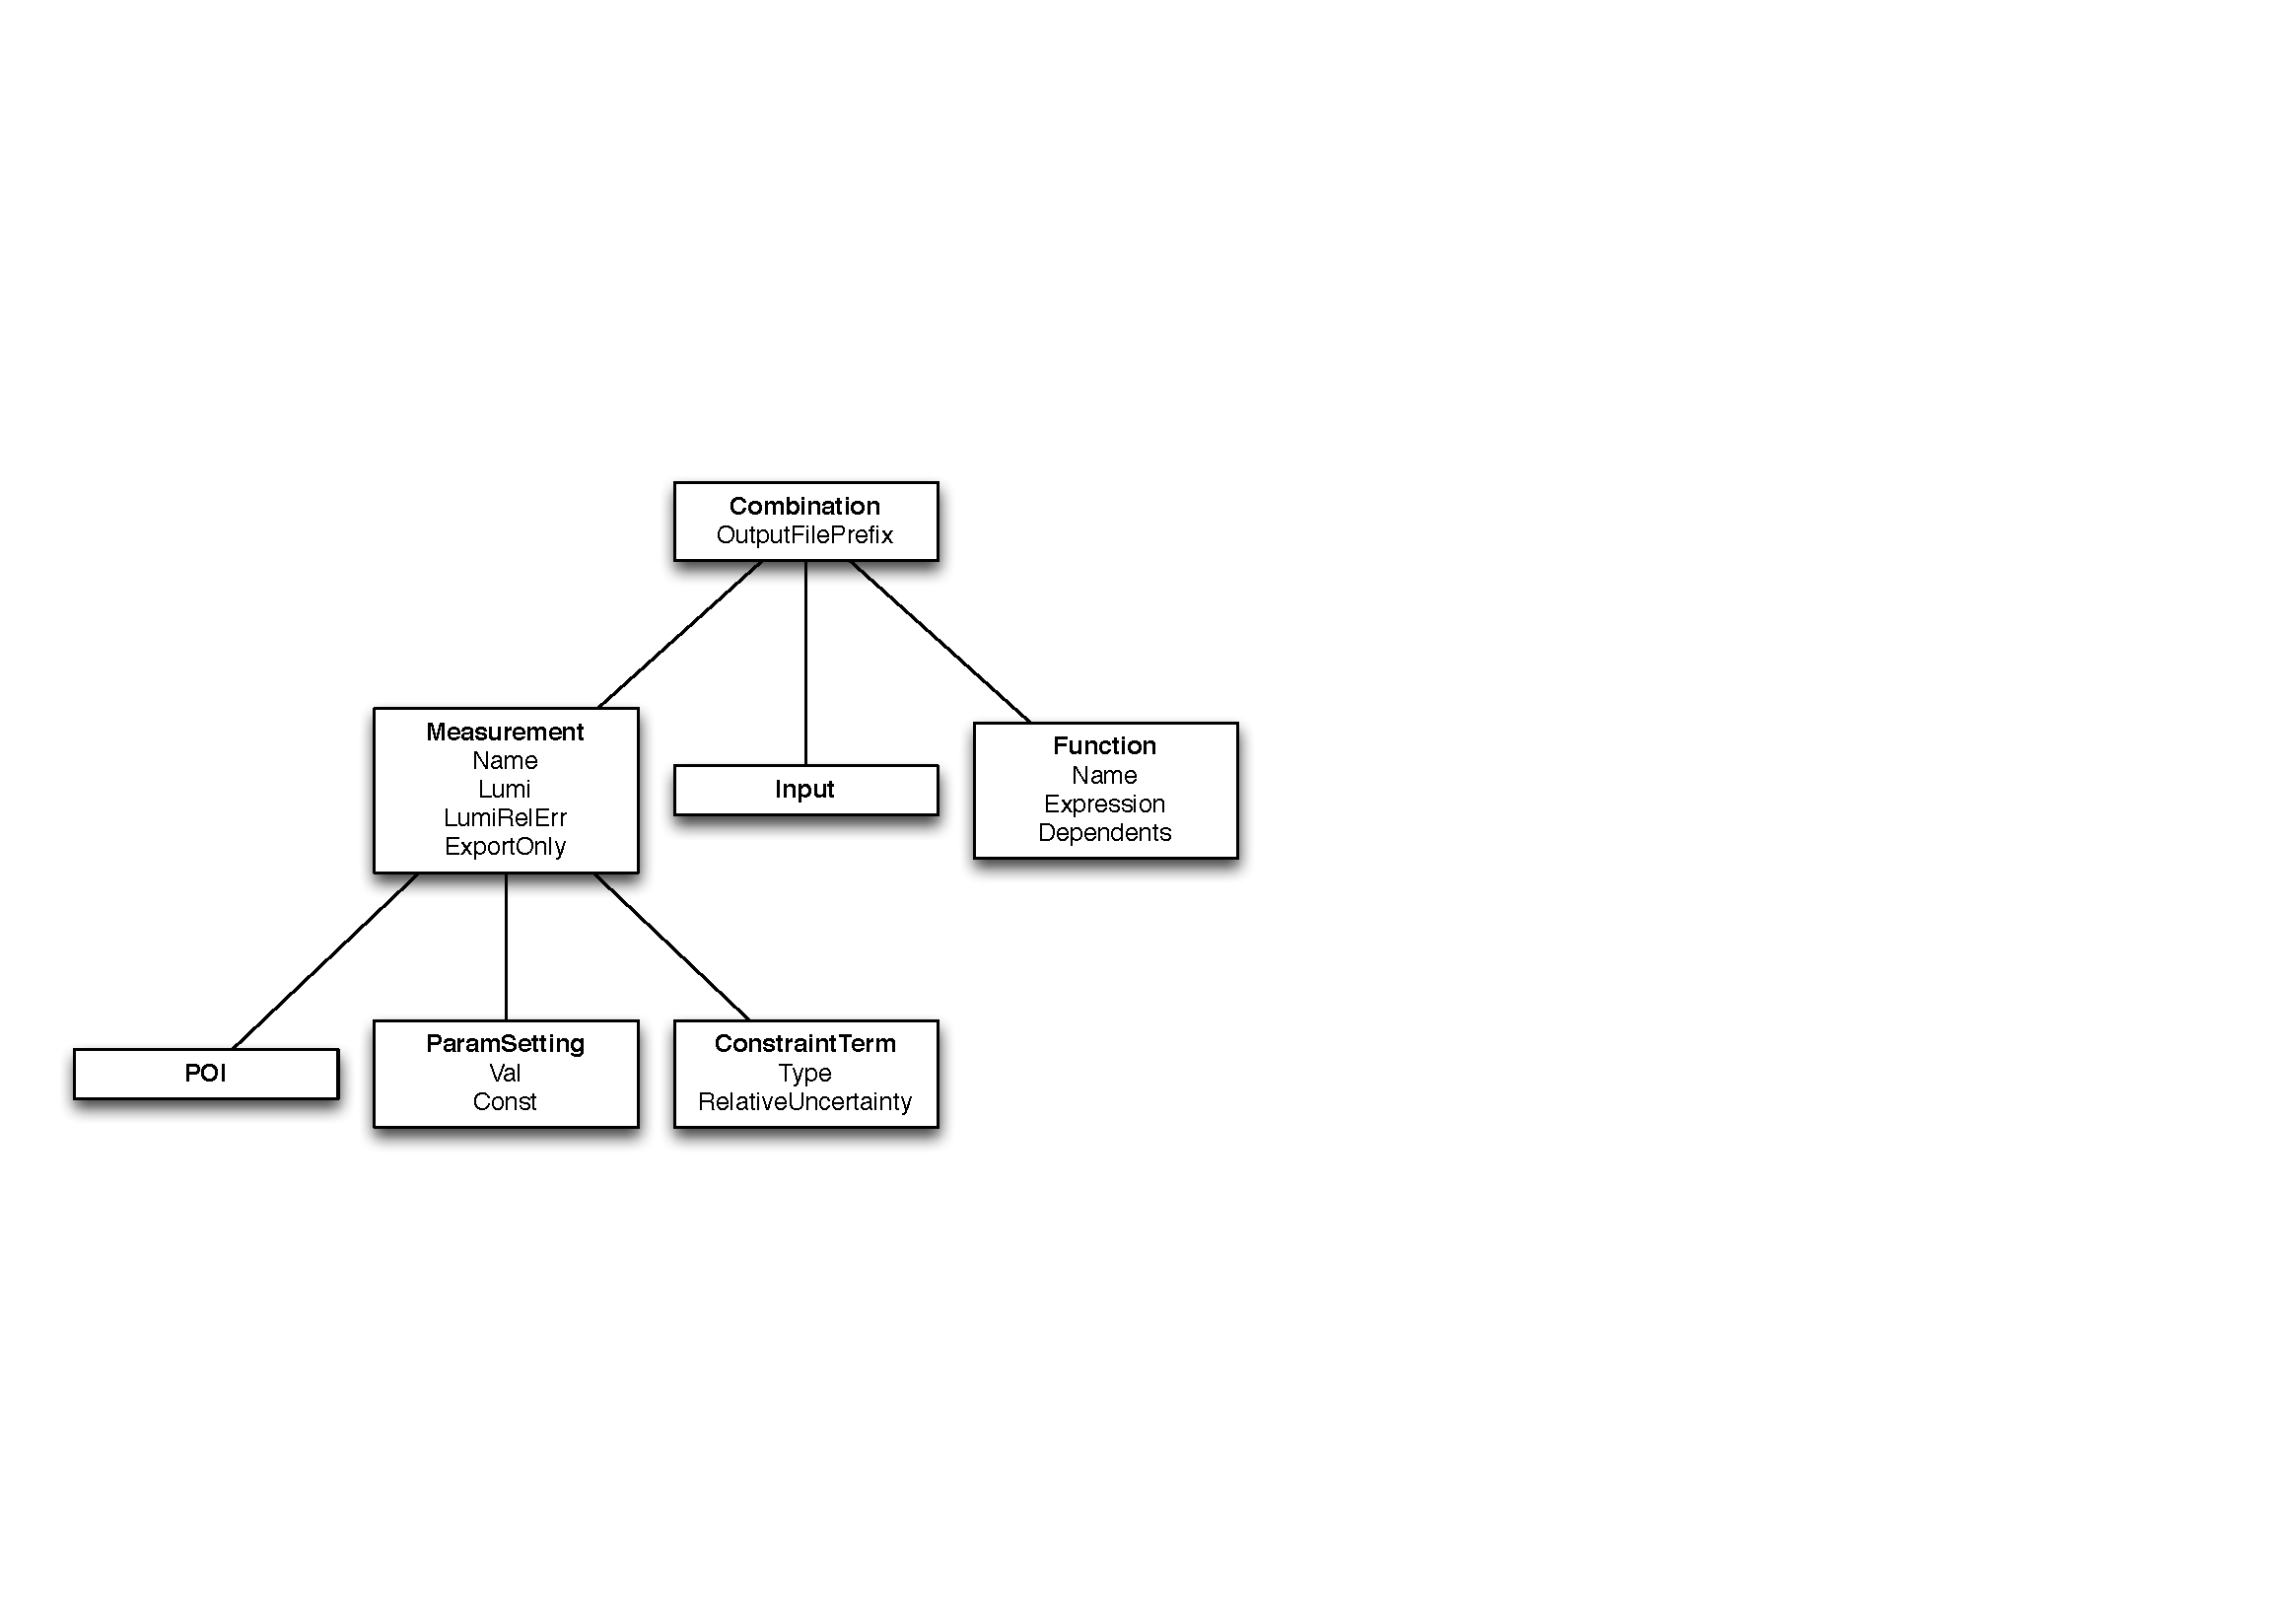
\includegraphics[width=.8\textwidth]{TopLevelXML.pdf}}
%\subfigure[][]{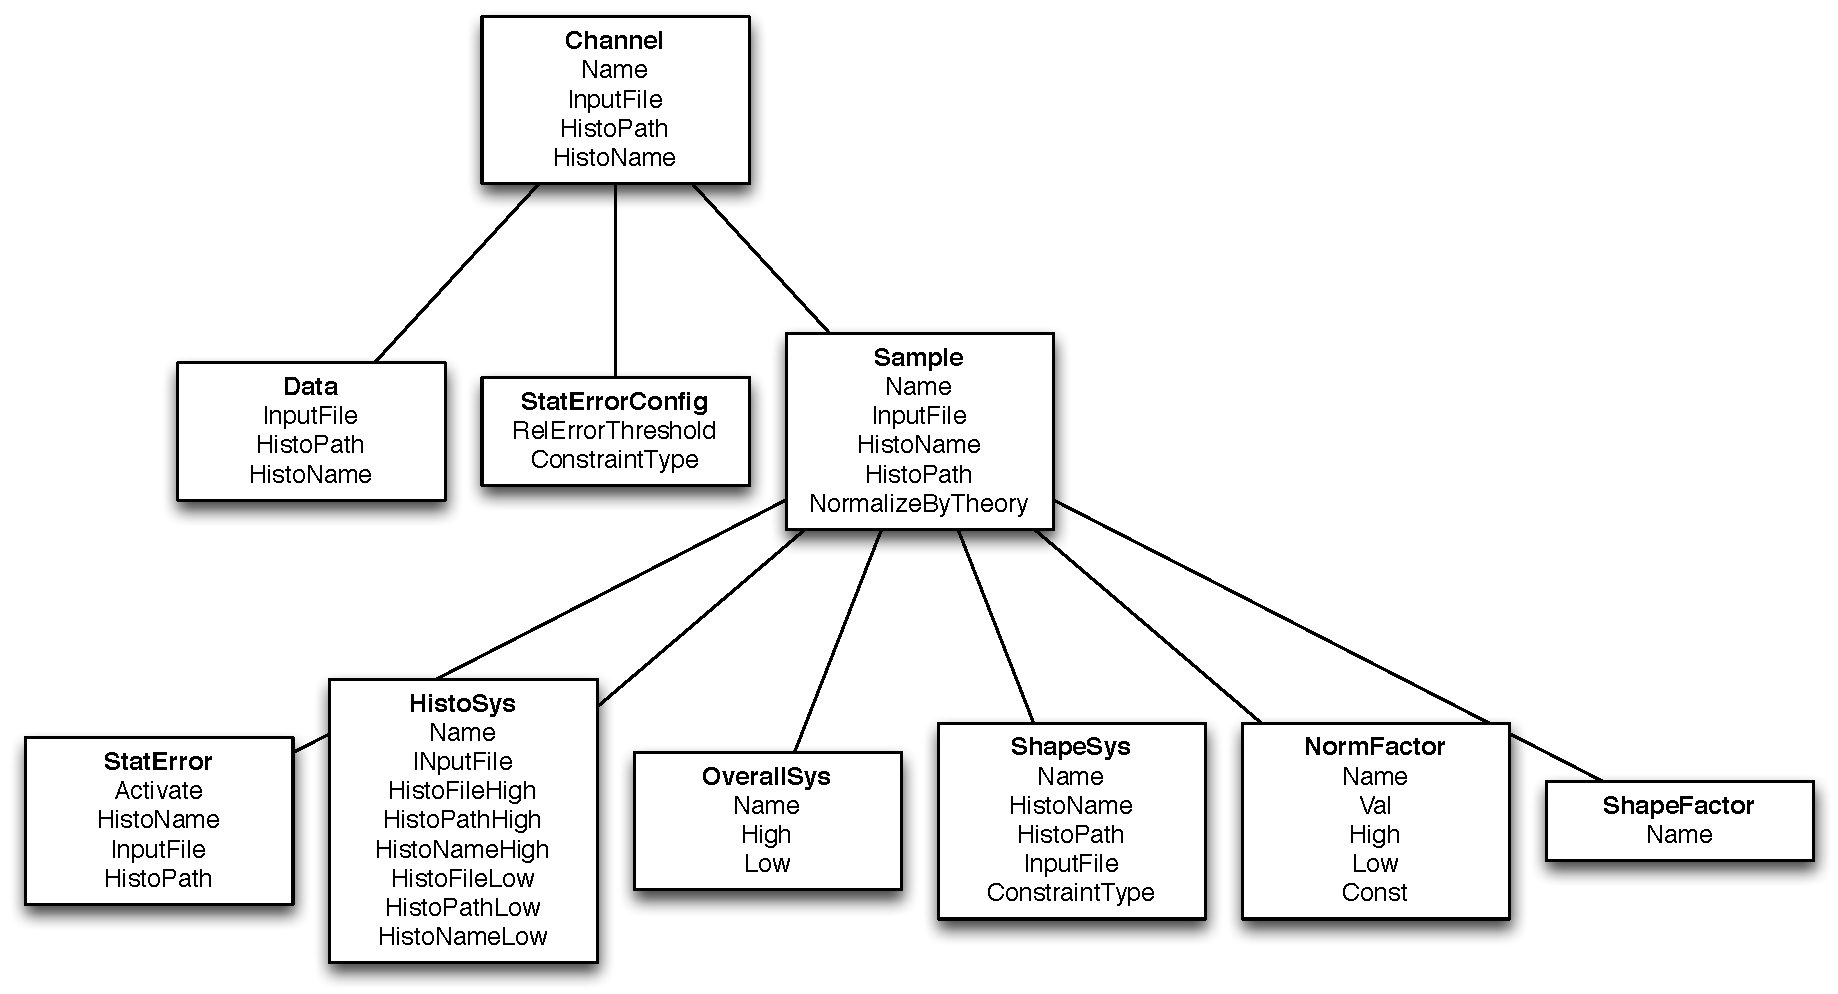
\includegraphics[width=.8\textwidth]{ChannelXML.pdf}}
\caption{The graphical representation of the XML schema.  Boxes are elements with name of element in bold and attributes listed below.  Elements without any attributes take their input as ``PCDATA", for example \texttt{<Input>someFile.xml</Input>}}
\label{fig:XML}
\end{center}
\end{figure}

Note, when using the {\tt HistFactory} the production modes $l$ and backgrounds $j$ correspond to a single XML {\tt Sample} element.  The   {\tt HistoName} attribute inside each sample element specifies the histogram with the  $\sigma_{ism}^0$.   The index $s='S$' is set by the {\tt Name} attribute of the {\tt Sample} element (eg. {\tt <Sample Name="S">}). Between the open {\tt <Sample>} and close {\tt </Sample>} one can add
\begin{itemize}
 \item An {\tt OverallSys} element where the {\tt Name="p"} attribute identifies which $\alpha_p$ is the source of the systematic and implies that the Gaussian constraint $f_p(a_p|\alpha_p)$ is present.  The {\tt High} attribute  corresponds to $\eta^+_{ps}$, eg when the source of the systematic is at +1$\sigma$ and $\alpha_p=1$.  Similarly, the {\tt Low} attribute corresponds to $\eta^-_{ps}$, eg when the source of the systematic is at -1$\sigma$ and $\alpha_p=-1$. The nominal value is $\eta^0_{ps}=1$ for the overall systematics. The distinction between the sign of the source $\alpha$ and the effect $\eta$ allows one to have anti-correlated systematics. The \HF\ is able to deal with asymmetric uncertainties as well, by using a  one of various interpolations.
 \item A {\tt NormFactor} element is used to introduce an overall constant factor into the expected number of events.  In the example below, the term $\mu=\sigma/\sigma_{SM}$ corresponds to the line {\tt <NormFactor Name="SigXsecOverSM">}.  In this case, the histograms were normalized to unity, so additional {\tt NormFactor} elements were used to give the overall cross-sections $\sigma_{s}$.
 \item A {\tt \HS\ } element is used to introduce shape systematics and the {\tt HistoNameHigh} and {\tt HistoNameLow} attributes have the variational histograms $\sigma_{psb}^+ $ and $\sigma_{psb}^- $ corresponding to $\alpha_p=+1$ and $\alpha_p=-1$, respectively.
\end{itemize}

\subsubsection{Normalization Conventions}



The nominal and variational histograms should all have the same normalization convention. There are a few conventions possible:
\begin{enumerate}
\item[] Option 1:
	\begin{itemize}
	 \item \texttt{Lumi="XXX"} in the measurement XML's element, where XXX is in fb$^{-1}$
	\item Histograms bins have units of fb
	\item Some samples have \NF\ that are all relative to prediction (eg. 1 is the nominal prediction)
	\end{itemize}
\item[] Option 2:
	\begin{itemize}
	\item \texttt{Lumi="1."} in the measurement XML's element
	\item Histograms are normalized to unity
	\item Each sample has a \NF\ that is the expected number of events in data
	\end{itemize}
\item[] Option 3:
	\begin{itemize}
	\item \texttt{Lumi="1"} in the measurement XML's element
	\item Histograms bins have units of number of events expected in data
	\item Some samples have \NF\ that are all relative to prediction (eg. 1 is the nominal prediction)
	\end{itemize}
\end{enumerate}
It's up to you. In the end, the expected number is the product Lumi$\times$NormFactor(s)$\times$BinContent corresponding to $\lambda_{cs}\phi_{cs}\sigma_{csb}$.  


\clearpage
%\subsubsection{The Resulting Model}
\begin{figure}[h]
\begin{center}
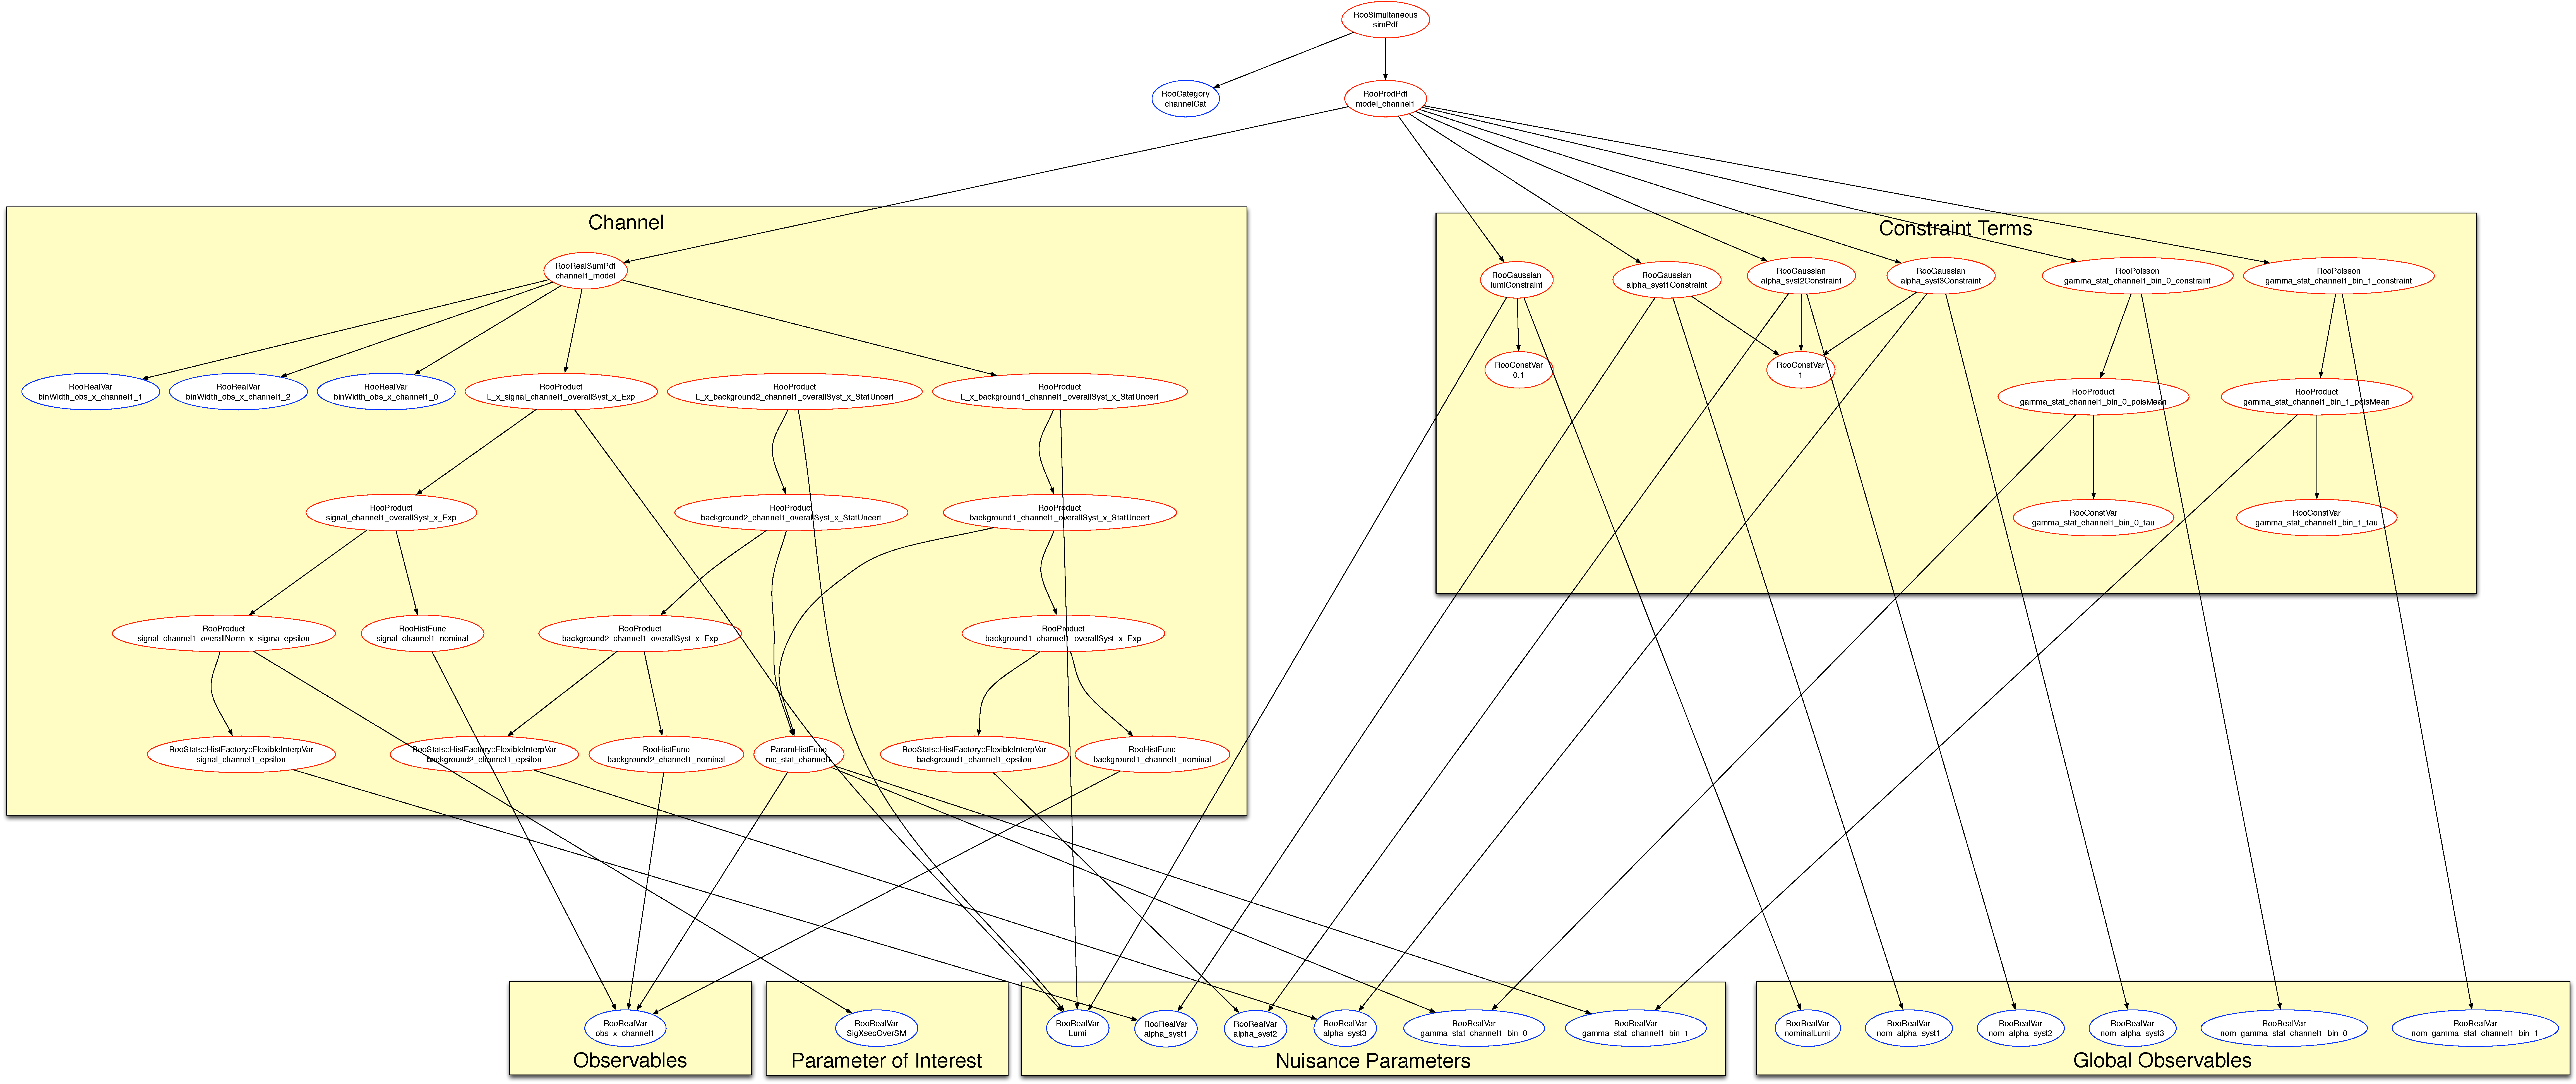
\includegraphics[width=.8\textheight,angle=90]{figures/histfactory/Example_graph}
\caption{A graphical representation of the resulting \RooFit\ model created from the standard example.  The nodes have been organized according to their role in the model.}
\label{fig:PDFGraph}
\end{center}
\end{figure}

\clearpage
\subsubsection{Usage of the HistFactory}

\flushleft{\textbf{ROOT installation}}

Download, install, and setup ROOT v5.28 or greater.  It is recommended to use one of the patch releases of v5.28 as the "standard form" described below was not available before the patch releases.
\begin{verbatim}
cd $ROOTSYS
source bin/thisroot.sh
\end{verbatim}
This will setup your \texttt{MANPATH} environment variable so that you can use the command line help.  

\flushleft{\textbf{prepareHistFactory}}

\begin{verbatim}
man prepareHistFactory
prepareHistFactory 
\end{verbatim}

       The command line executable \texttt{prepareHistFactory [dir\_name]}  is  a simple script that prepares a working area (and creates the directory
       dir\_name if specified).  Within the directory dir\_name, it creates a results/, data/, and  config/  directory relative to the given path.  It also copies the HistFactorySchema.dtd and example XML files into the config/ directory.  Additionally, it copies a root file into  the  data/
       directory  for  use  with  the  examples.   Once  this is done, one is ready to run the example
       hist2workspace input.xml or edit the XML files for a new project.


\flushleft{\textbf{hist2workspace}}

\begin{verbatim}
man hist2workspace
hist2workspace config/example.xml
\end{verbatim}

       The command line executable \texttt{hist2workspace [option] [input xml]} is a utility to create RooFit/RooStats workspace from histograms

OPTIONS:
\begin{itemize}
      \item \texttt{-standard\_form}  default model (from v5.28.00a and beyond), which creates an extended PDF that interpolates between RooHistFuncs.  This is much faster for models with many bins and uses significantly less memory.
       \item \texttt{-number\_counting\_form} this was the original model in 5.28 (without patches). It uses a  Poisson
       for  each  bin of the histogram.  This can become slow and memory intensive when there are many
       bins.
\end{itemize}


\subsubsection{Usage with RooStats tools}

Once one runs \texttt{hist2workspace} on an XML file there will be output root and eps files in the results directory.  The files are named
\begin{verbatim}
   results/[Prefix]_[Channel]_[Measurement]_model.root
\end{verbatim}
where Prefix is specified in the \texttt{<Combination>} element in the top-level XML file, for example:
\begin{verbatim}
   <Combination OutputFilePrefix="./results/example" Mode="comb" >
\end{verbatim}
Measurement is specified in each of the \texttt{<Measurement>} elements in the top-level XML file
\begin{verbatim}
   <Measurement Name="AllSYS" ...>
\end{verbatim}
and Channel  is "combined" for the combined model, but a model file is exported for each individual channel as well using the name taken from the  \texttt{<Channel>} element of the corresponding channel's XML file
\begin{verbatim}
  <Channel Name="channelEle" ...>
\end{verbatim}


These root files have inside a RooWorkspace which contains a RooDataSet and a ModelConfig that can be used with standard RooStats tools (see for example \texttt{\$ROOTSYS/tutorials/RooStats/Standard*Demo.C}


\newpage
%%%%%%%%%%%%%%%%%%%%%%%%%%%%%%%%%%%%%%%%%%%%%%%%%
\subsection{Interpolation \& Constraints}

The treatment of systematic uncertainties is subtle, particularly when one wishes to take into account the correlated effect of multiple sources of systematic uncertainty across many signal and background samples.   
The most important conceptual issue is that we separate the source of the uncertainty (for instance the uncertainty in the calorimeter's response to jets) from its effect on an individual signal or background sample (eg. the change in the acceptance and shape of a $W$+jets background).  In particular, the same source of uncertainty has a different effect on the various signal and background samples~\footnote{Here we suppress the channel index $c$ on $\eta_{cs}$ and $\sigma_{cab}$}.  The effect of these ``$\pm 1\sigma$'' variations about the nominal predictions $\eta_s^0=1$  and $\sigma_{sb}^0$ is quantified by dedicated studies that provide $\eta_{sp}^\pm$ and $\sigma_{spb}^\pm$.  The result of these studies can be arranged in tables like those below.  The main purpose of the \HF\ XML schema is to represent these tables.

%That is to say that there is a nuisance parameter $\alpha_p$ associated with a particular source of systematic effect, for instance $\alpha_{\rm JES}$ for an uncertain jet energy scale.  

\begin{table}[h]
\center
\begin{tabular}{l | c c c}
Syst & Sample 1 & $\dots$ & Sample N \\ \hline
Nominal Value & $\eta_{s=1}^0=1$ & \dots & $\eta_{s=N}^0=1$\\\hline
$p$=\OS\ 1 & $\eta_{p=1,s=1}^+$, \;$\eta_{p=1,s=1}^-$ & \dots & $\eta_{p=1,s=N}^+$,\; $\eta_{p=1,s=N}^-$\\ 
$\vdots$ & $\vdots$ & $\ddots$ & $\vdots$ \\
$p$=\OS\ M & $\eta_{p=M,s=1}^+$, $\eta_{p=M,s=1}^-$ & \dots & $\eta_{p=M,s=N}^+$, $\eta_{p=M,s=N}^-$\\ \hline
Net Effect & $\eta_{s=1}(\vec{\alpha})$ & \dots & $\eta_{s=N}(\vec{\alpha})$
\end{tabular}
\caption{Tabular representation of sources of uncertainties that produce a correlated effect in the normalization individual samples (eg. OverallSys).  The $\eta^+_{ps}$ represent histogram when $\alpha_s=1$ and are inserted into the \texttt{High} attribute of the \OS\  XML element.  Similarly, the $\eta^-_{ps}$ represent histogram when $\alpha_s=-1$ and are inserted into the \texttt{Low} attribute of the \OS\  XML element. Note, this does not imply that $\eta^+ > \eta^-$, the $\pm$ superscript correspond to the variation in the source of the systematic, not the resulting effect.}
\end{table}

\begin{table}[h]
\center
\begin{tabular}{l | c c c}
Syst & Sample 1 & $\dots$ & Sample N \\ \hline
Nominal Value & $\sigma_{s=1,b}^0$ & \dots & $\sigma_{s=N,b}^0$\\\hline
$p$=\HS\  1\;\; & $\sigma_{p=1,s=1,b}^+$, $\sigma_{p=1,s=1,b}^-$ & \dots & $\sigma_{p=1,s=N,b}^+$, $\sigma_{p=1,s=N,b}^-$\\ 
$\vdots$ & $\vdots$ & $\ddots$ & $\vdots$ \\
$p$=\HS\  M \;\;\;\;& $\sigma_{p=M,s=1,b}^+$, \;\;$\sigma_{p=M,s=1,b}^-$ \;\;& \dots & $\sigma_{p=M,s=N,b}^+$, \;\; $\sigma_{p=M,s=N,b}^-$\;\;\\ \hline
Net Effect & $\sigma_{s=1,b}(\vec{\alpha})$ & \dots & $\sigma_{s=N,b}(\vec{\alpha})$
\end{tabular}
\caption{Tabular representation of sources of uncertainties that produce a correlated effect in the normalization and shape individual samples (eg. \HS\ ).  The $\sigma^+_{psb}$ represent histogram when $\alpha_s=1$ and are inserted into the \texttt{HighHist} attribute of the \HS\  XML element.  Similarly, the $\sigma^-_{psb}$ represent histogram when $\alpha_s=-1$ and are inserted into the \texttt{LowHist} attribute of the \HS\  XML element.   }
\end{table}

Once one has tabulated the effects of the individual sources of systematic uncertainty as above, one must address two related issues to form a likelihood parametrized with continuous nuisance parameters.  
First, one must provide an interpolation algorithm to interpolate to define $\eta_{s}(\vec{\alpha})$ and $\sigma_{sb}(\vec{\alpha})$.  Secondly, one must incorporate constraint terms on the $\alpha_p$ to reflect that the uncertain parameter has been estimated with some uncertainty by an auxiliary measurement.  A strength of the histogram template based approach (compared to parametrized analytic functions) is that the effect of individual systematics are tracked explicitly; however, the ambiguities associated to the interpolation and constraints are a weakness.

\subsubsection{Interpolation Options}
\label{S:Interpolation}


For each sample, one can interpolate and extrapolate from the nominal prediction $\eta_s^0=1$ and the variations $\eta^\pm_{ps}$ to produce a parametrized $\eta_s(\vec{\alpha})$.   Similarly, one can interpolate and extrapolate from the nominal shape $\sigma_{sb}^0$ and the variations $\sigma^\pm_{psb}$ to produce a parametrized $\sigma_{sb}(\vec{\alpha})$.  We choose to parametrize $\alpha_p$ such that $\alpha_p=0$ is the nominal value of this parameter, $\alpha_p=\pm 1$ are the ``$\pm 1\sigma$ variations''.  Needless to say, there is a significant amount of ambiguity in these interpolation and extrapolation procedures and they must be handled with care.  In the future the \texttt{HistFactory} may support other types of shape interpolation, but as of ROOT 5.32 the shape interpolation is a 'vertical' style interpolation that is treated independently per-bin. Four interpolation strategies are described below and can be compared in Fig~\ref{fig:interp1d}.  
%\newpage
%%%%%%%%%
\flushleft{\bf Piecewise Linear (InterpCode=0)}

The piecewise-linear interpolation strategy is defined as
\begin{equation}
\eta_s ({\boldsymbol \alpha}) = 1+\sum_{p\in\textrm{Syst}} I_{\rm lin.}(\alpha_p; 1, \eta_{sp}^+, \; \eta_{sp}^- ) 
\end{equation}
and for shape interpolation it is
\begin{equation}
\sigma_{sb} ({\boldsymbol \alpha}) = \sigma_{sb}^0 + \sum_{p\in\textrm{Syst}} I_{\rm lin.}(\alpha_p;  \sigma_{sb}^0, \sigma_{psb}^+ ,\;
\sigma_{psb}^- )  
\end{equation}
with
\begin{equation}
 I_{\rm lin.}(\alpha;  I^0, I^+,I^- ) =
 \begin{cases}
     \alpha (I^+  -  I^0) &  \text{$\alpha\ge 0$} \\
     \alpha (I^0  -I^-)  &  \text{$\alpha<0$ }
 \end{cases}
\end{equation}

\textsc{Pros:} This approach is the most straightforward of the interpolation strategies.

\textsc{Cons:} It has two negative features.  First, there is a kink (discontinuous first derivative) at $\alpha=0$ (see Fig~\ref{fig:interp1d}(b-d)), which can cause some difficulties for numerical minimization packages such as \texttt{Minuit}.  Second, the interpolation factor can extrapolate to negative values.  For instance, if $\eta^-=0.5$ then  we have $\eta(\alpha)<0$  when $\alpha<-2$  (see Fig~\ref{fig:interp1d}(c)).  

Note that one could have considered the simultaneous variation of $\alpha_{p}$ and $\alpha_{p'}$ in a multiplicative way (see for example, Fig~\ref{fig:interp2d}).  The multiplicative accumulation is not an option currently.

Note that this is the default convention for $\sigma_{sb}(\vec{\alpha})$ (ie. \HS\ ).

%%%%%%%%%
\flushleft{\bf Piecewise Exponential (InterpCode=1)}

The piecewise exponential interpolation strategy is defined as
\begin{equation}
\eta_s ({\boldsymbol \alpha}) = \prod_{p\in\textrm{Syst}} I_{\rm exp.}(\alpha_p; 1,\eta_{sp}^+, \; \eta_{sp}^- ) 
\end{equation}
and for shape interpolation it is
\begin{equation}
\sigma_{sb} ({\boldsymbol \alpha}) = \sigma_{sb}^0 \prod_{p\in\textrm{Syst}} I_{\rm exp.}(\alpha_p;  \sigma_{sb}^0, \sigma_{psb}^+ ,\;
\sigma_{psb}^- )  
\end{equation}
with
\begin{equation}
 I_{\rm exp.}(\alpha;  I^0, I^+,I^- ) =
 \begin{cases}
     (I^+/I_0)^ \alpha  &  \text{$\alpha\ge 0$} \\
     (I^-/I_0)^{-\alpha}  &  \text{$\alpha<0$ }
 \end{cases}
\end{equation}

\textsc{Pros:} This approach ensures that $\eta(\alpha)\ge 0$ (see Fig~\ref{fig:interp1d}(c)) and for small response to the uncertainties it has the same linear behavior near $\alpha\sim 0$ as the piecewise linear interpolation (see Fig~\ref{fig:interp1d}(a)).

\textsc{Cons:} It has two negative features.  First, there is a kink (discontinuous first derivative) at $\alpha=0$, which can cause some difficulties for numerical minimization packages such as \texttt{Minuit}.  Second, for large uncertainties it develops a different linear behavior compared to the piecewise linear interpolation.  In particular, even if the systematic has a symmetric response (ie. $\eta^+-1 = 1-\eta^-$) the interpolated response will develop a kink for large response to the uncertainties  (see Fig~\ref{fig:interp1d}(c)).

Note that the one could have considered the simultaneous variation of $\alpha_{p}$ and $\alpha_{p'}$ in an additive way, but this is not an option currently.

Note, that when paired with a Gaussian constraint on $\alpha$ this is equivalent to  linear interpolation and a log-normal constraint in $\ln(\alpha)$.  This is the default strategy for normalization uncertainties $\eta_{s}(\vec{\alpha})$ (ie. \OS\ ) and is the standard convention for normalization uncertainties in the LHC Higgs Combination Group.  In the future, the default may change to the Polynomial Interpolation and Exponential Extrapolation described below.

%%%%%%%%%
\flushleft{\bf Quadratic Interpolation and Linear Extrapolation (InterpCode=2)}

The quadratic interpolation and linear extrapolation strategy is defined as

\begin{equation}
\eta_s ({\boldsymbol \alpha}) = 1+\sum_{p\in\textrm{Syst}} I_{\rm quad.|lin.}(\alpha_p; 1, \eta_{sp}^+, \; \eta_{sp}^- ) 
\end{equation}
and for shape interpolation it is
\begin{equation}
\sigma_{sb} ({\boldsymbol \alpha}) = \sigma_{sb}^0 + \sum_{p\in\textrm{Syst}} I_{\rm quad.|lin.}(\alpha_p;  \sigma_{sb}^0, \sigma_{psb}^+ ,\;
\sigma_{psb}^- )  
\end{equation}
 with
\begin{equation}
 I_{\rm quad.|lin.}(\alpha;  I^0, I^+,I^- ) =
 \begin{cases}
   (b+2a)(\alpha-1)  &  \text{$\alpha>1$} \\
     a\alpha^2 + b\alpha                        &  \text{$|\alpha|\le1$} \\
     (b-2a)(\alpha+1)  &  \text{$\alpha<-1$ }
 \end{cases}
\end{equation}
and 
\begin{eqnarray}
a = \half (I^+ + I^-) -I^0 \hspace{.5in} \textrm{and} \hspace{.5in} b= \half(I^+ - I^-) \; .
\end{eqnarray}


\textsc{Pros:} This approach avoids the kink (discontinuous first derivative) at $\alpha=0$ (see middle panel of Fig~\ref{fig:interp1d}), which can cause some difficulties for numerical minimization packages such as \texttt{Minuit}.

\textsc{Cons:} It has a few negative features.  First, in the case that both the response to both positive and negative variations have the same sign of effect relative to the nominal (ie. $(\eta^+ -1)(\eta^- -1)>0$), the quadratic interpolation can lead to an an intermediate value with the opposite effect.  For example,  Fig~\ref{fig:interp1d}(b) shows a case where $\eta(\alpha=-0.3)<1$ while $\eta^\pm>0$.  Second, when the positive and negative variations have opposite signs, the extrapolation can reverse the trend.  For example, Fig~\ref{fig:interp1d}(d) shows an example for $\eta^-=0.95$ and $\eta^+=1.5$ where for $\alpha\lesssim 1.5$ we have the reversal $\eta(\alpha)>1$. Third, the interpolation factor can extrapolate to negative values.  For instance, if $\eta^-=0.5$ then  we have $\eta(\alpha)<0$  when $\alpha<-2$  (see Fig~\ref{fig:interp1d}(c)).  

Note that one could have considered the simultaneous variation of $\alpha_{p}$ and $\alpha_{p'}$ in a multiplicative way (see for example, Fig~\ref{fig:interp2d}).  The multiplicative accumulation is not an option currently.

%%%%%%%%%
\flushleft{\bf Polynomial Interpolation and Exponential Extrapolation (InterpCode=4)}

The strategy of this interpolation option is to use the piecewise exponential extrapolation as above with a polynomial interpolation that matches $\eta(\alpha=\pm\alpha_0)$, $d\eta/d\alpha |_{\alpha=\pm\alpha_0}$, and $d^2\eta/d\alpha^2 |_{\alpha=\pm\alpha_0}$ and the boundary $\pm\alpha_0$ is defined by the user (with default $\alpha_0=1$).  
\begin{equation}
\eta_s ({\boldsymbol \alpha}) = \prod_{p\in\textrm{Syst}} I_{\rm poly|exp.}(\alpha_p; 1,\eta_{sp}^+, \; \eta_{sp}^- , \alpha_0) 
\end{equation}
%and for shape interpolation it is
%\begin{equation}
%\sigma_{sb} ({\boldsymbol \alpha}) = \sigma_{sb}^0 \prod_{p\in\textrm{Syst}} I_{\rm poly|exp.}(\alpha_p;  \sigma_{sb}^0, \sigma_{psb}^+ ,\;
%\sigma_{psb}^- )  
%\end{equation}
with
\begin{equation}
 I_{\rm poly|exp.}(\alpha;  I^0, I^+,I^- , \alpha_0) =
 \begin{cases}
      (I^+/I_0)^ \alpha  &  \text{$\alpha\ge \alpha_0$} \\
     1+\sum_{i=1}^6 a_i \alpha^i  &  \text{$|\alpha|< \alpha_0$} \\
      (I^-/I_0)^{-\alpha}  &  \text{$\alpha\le-\alpha_0$ }
 \end{cases}
\end{equation}
and the $a_i$ are fixed by the boundary conditions described above.

\textsc{Pros:} This approach avoids the kink (discontinuous first and second derivatives) at $\alpha=0$ (see Fig~\ref{fig:interp1d}(b-d)), which can cause some difficulties for numerical minimization packages such as \texttt{Minuit}.  This approach ensures that $\eta(\alpha)\ge 0$ (see Fig~\ref{fig:interp1d}(c)). 


\textbf{Note}: This option is not available in ROOT 5.32.00, but is available for normalization uncertainties (OverallSys) in the subsequent patch releases.  In future releases, this may become the default.


\begin{figure}[h]
\begin{center}
\subfigure[][]{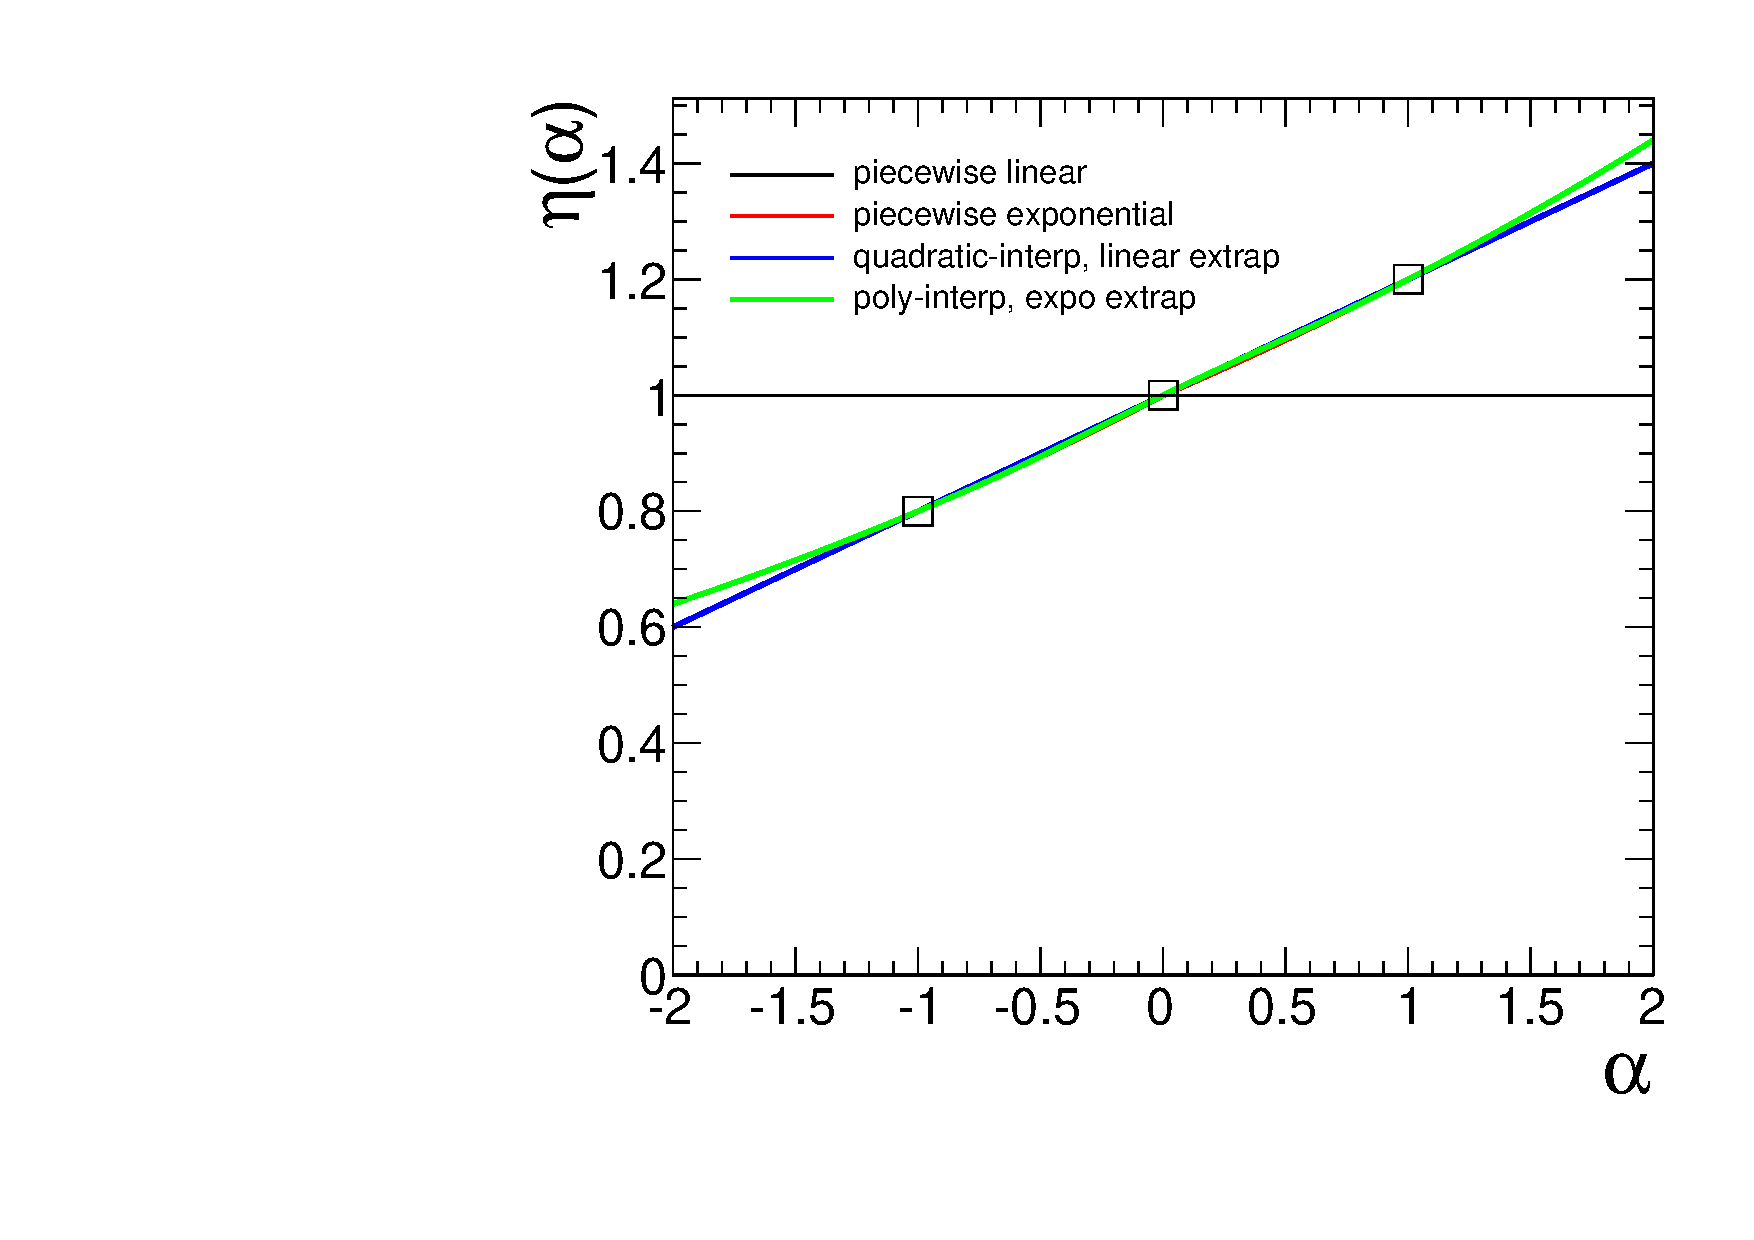
\includegraphics[width=.4\textwidth]{figures/histfactory/interpOption_8_12.pdf}}
\subfigure[][]{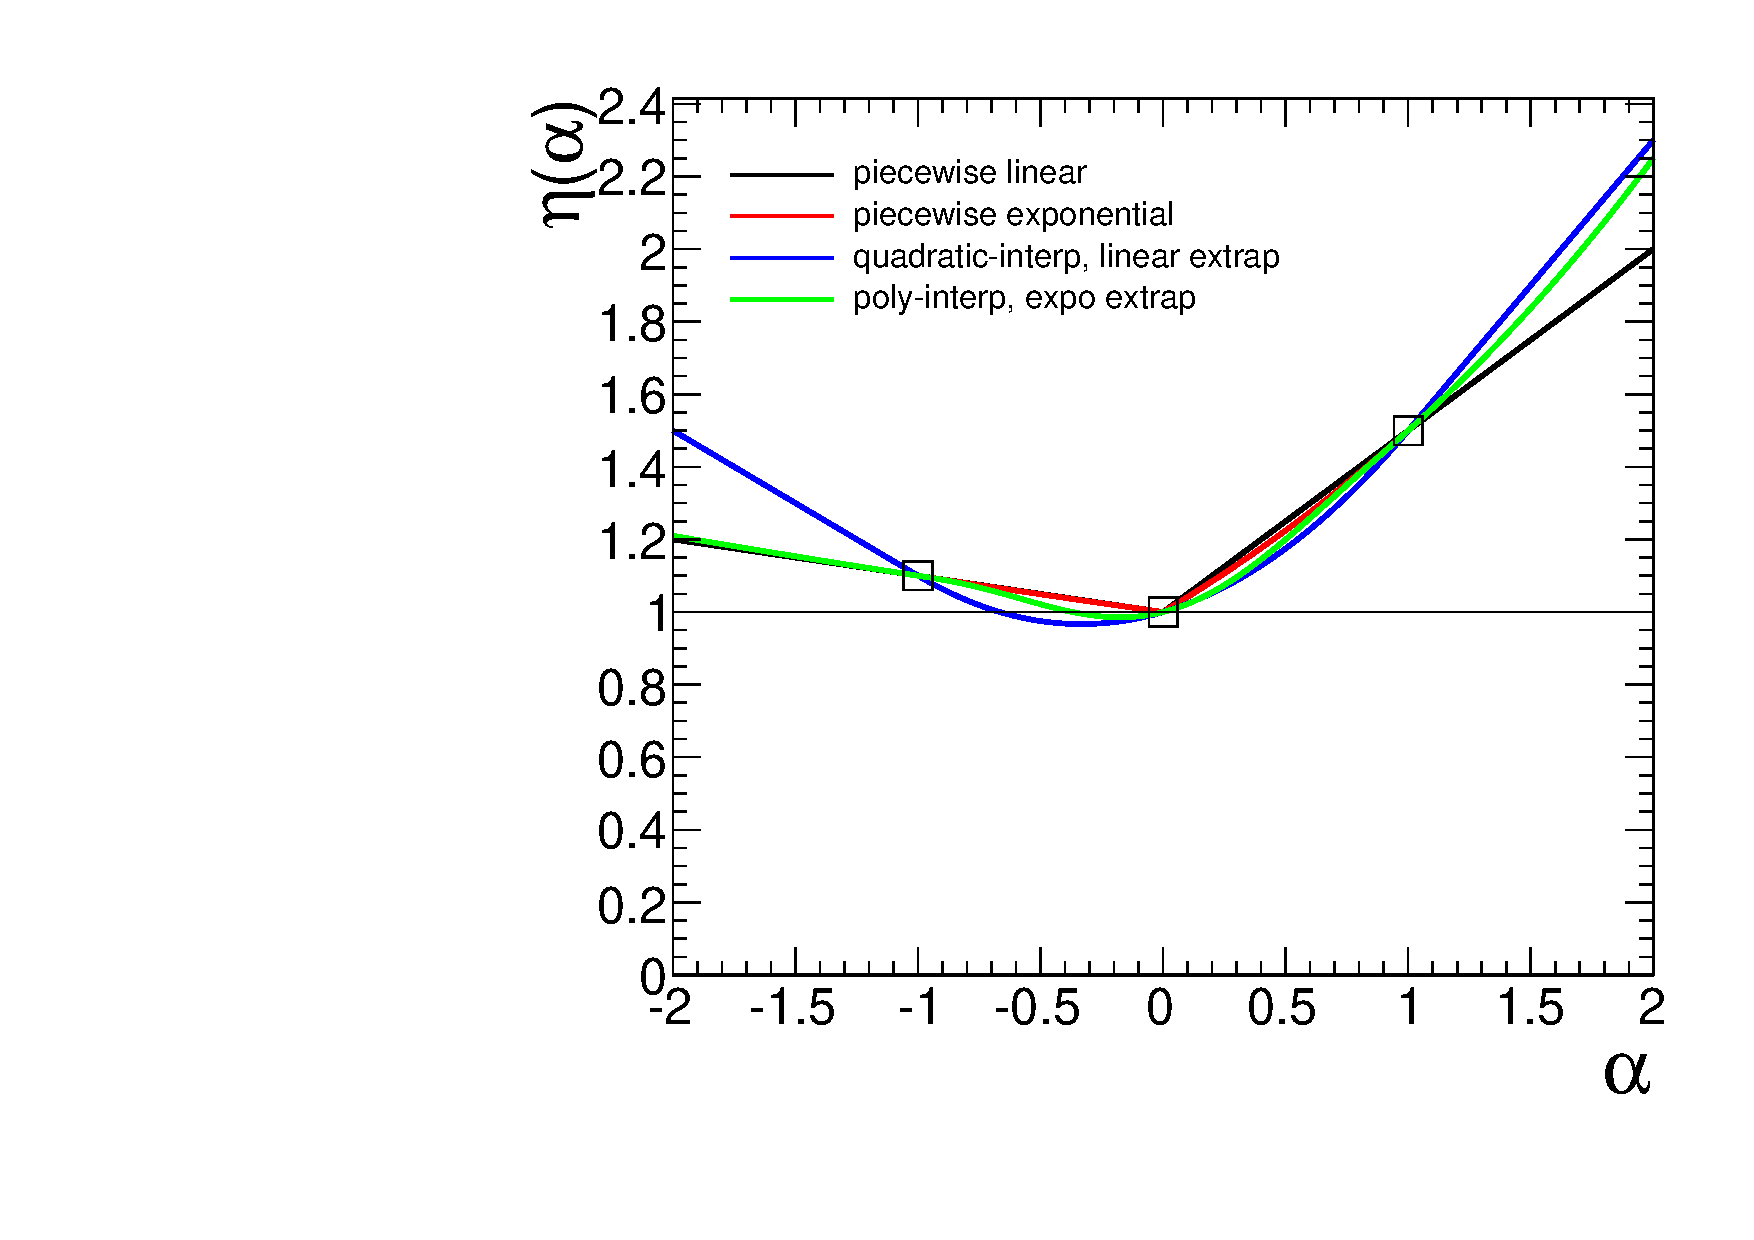
\includegraphics[width=.4\textwidth]{figures/histfactory/interpOption_11_15.pdf}}
\subfigure[][]{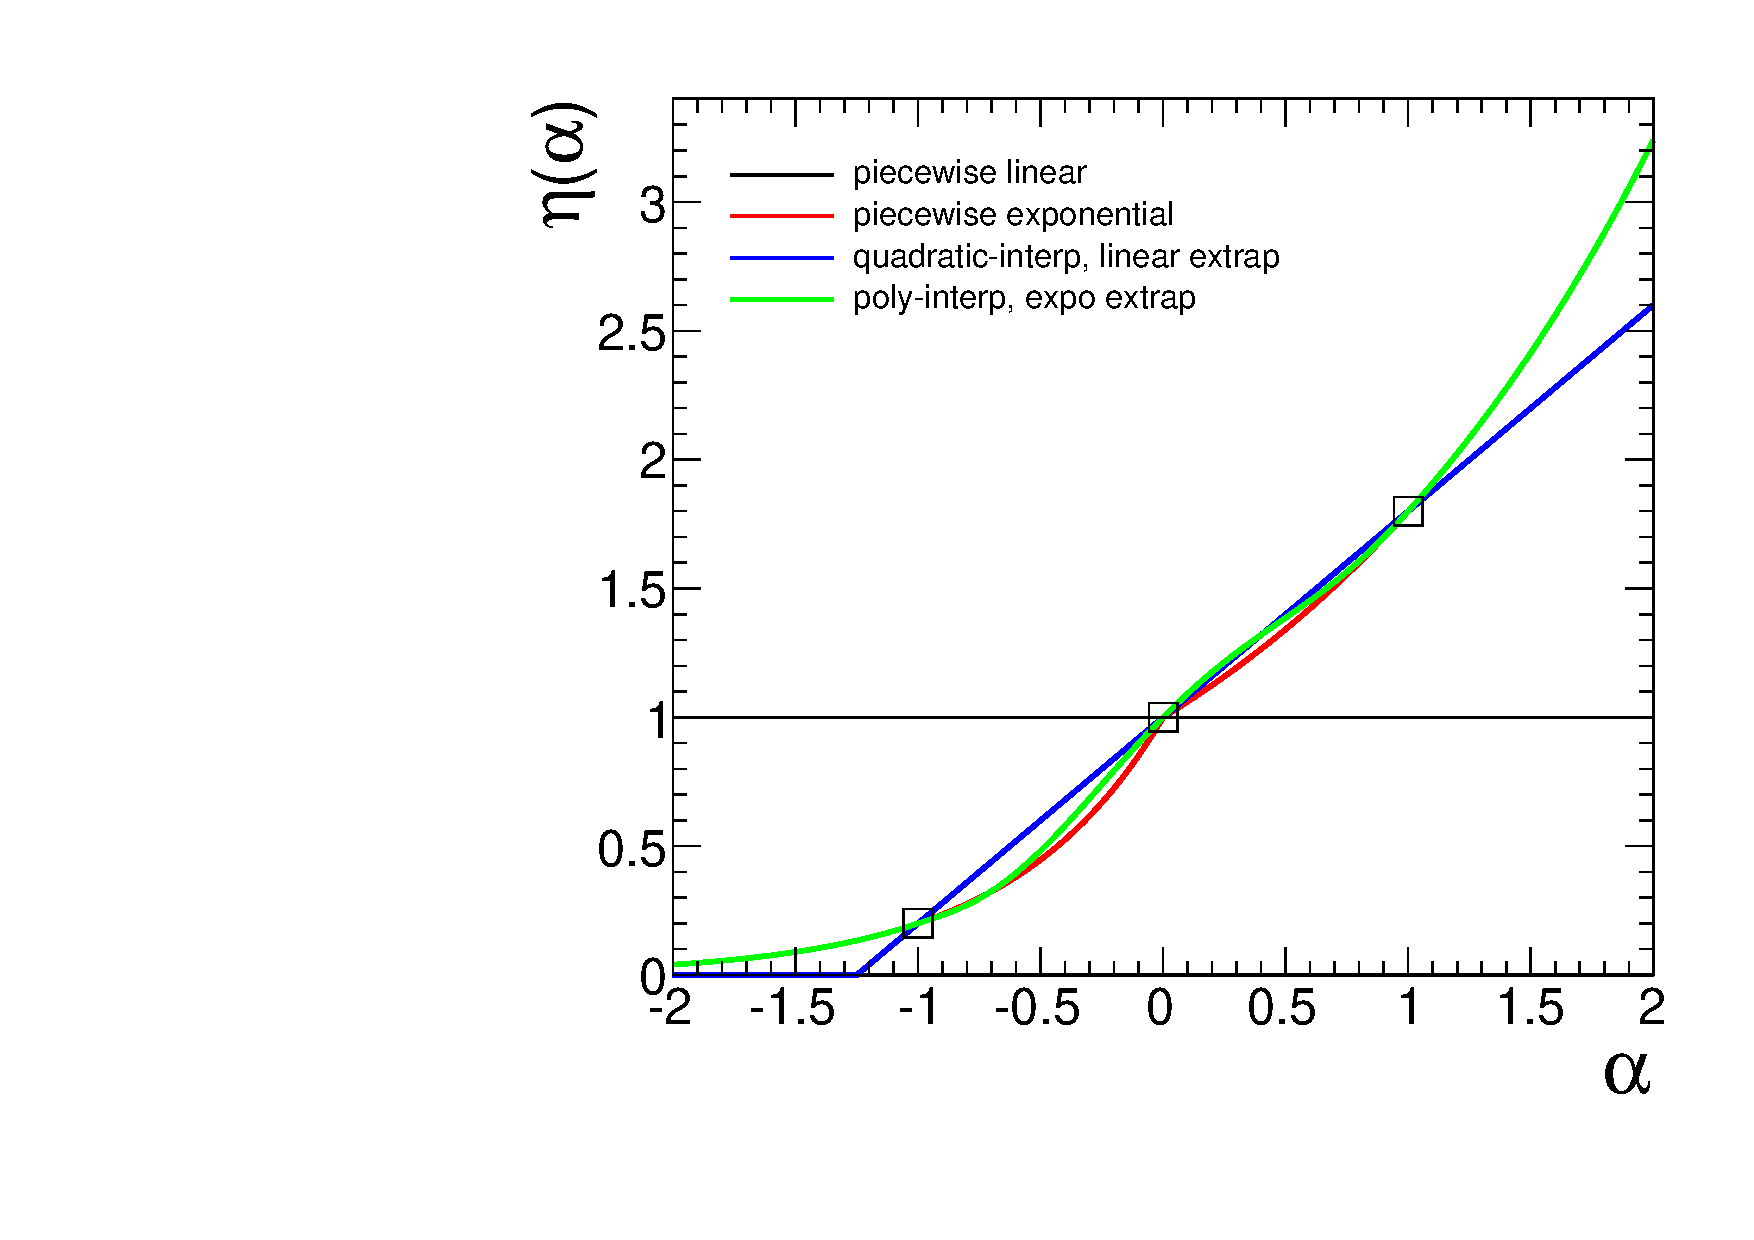
\includegraphics[width=.4\textwidth]{figures/histfactory/interpOption_2_18.pdf}}
\subfigure[][]{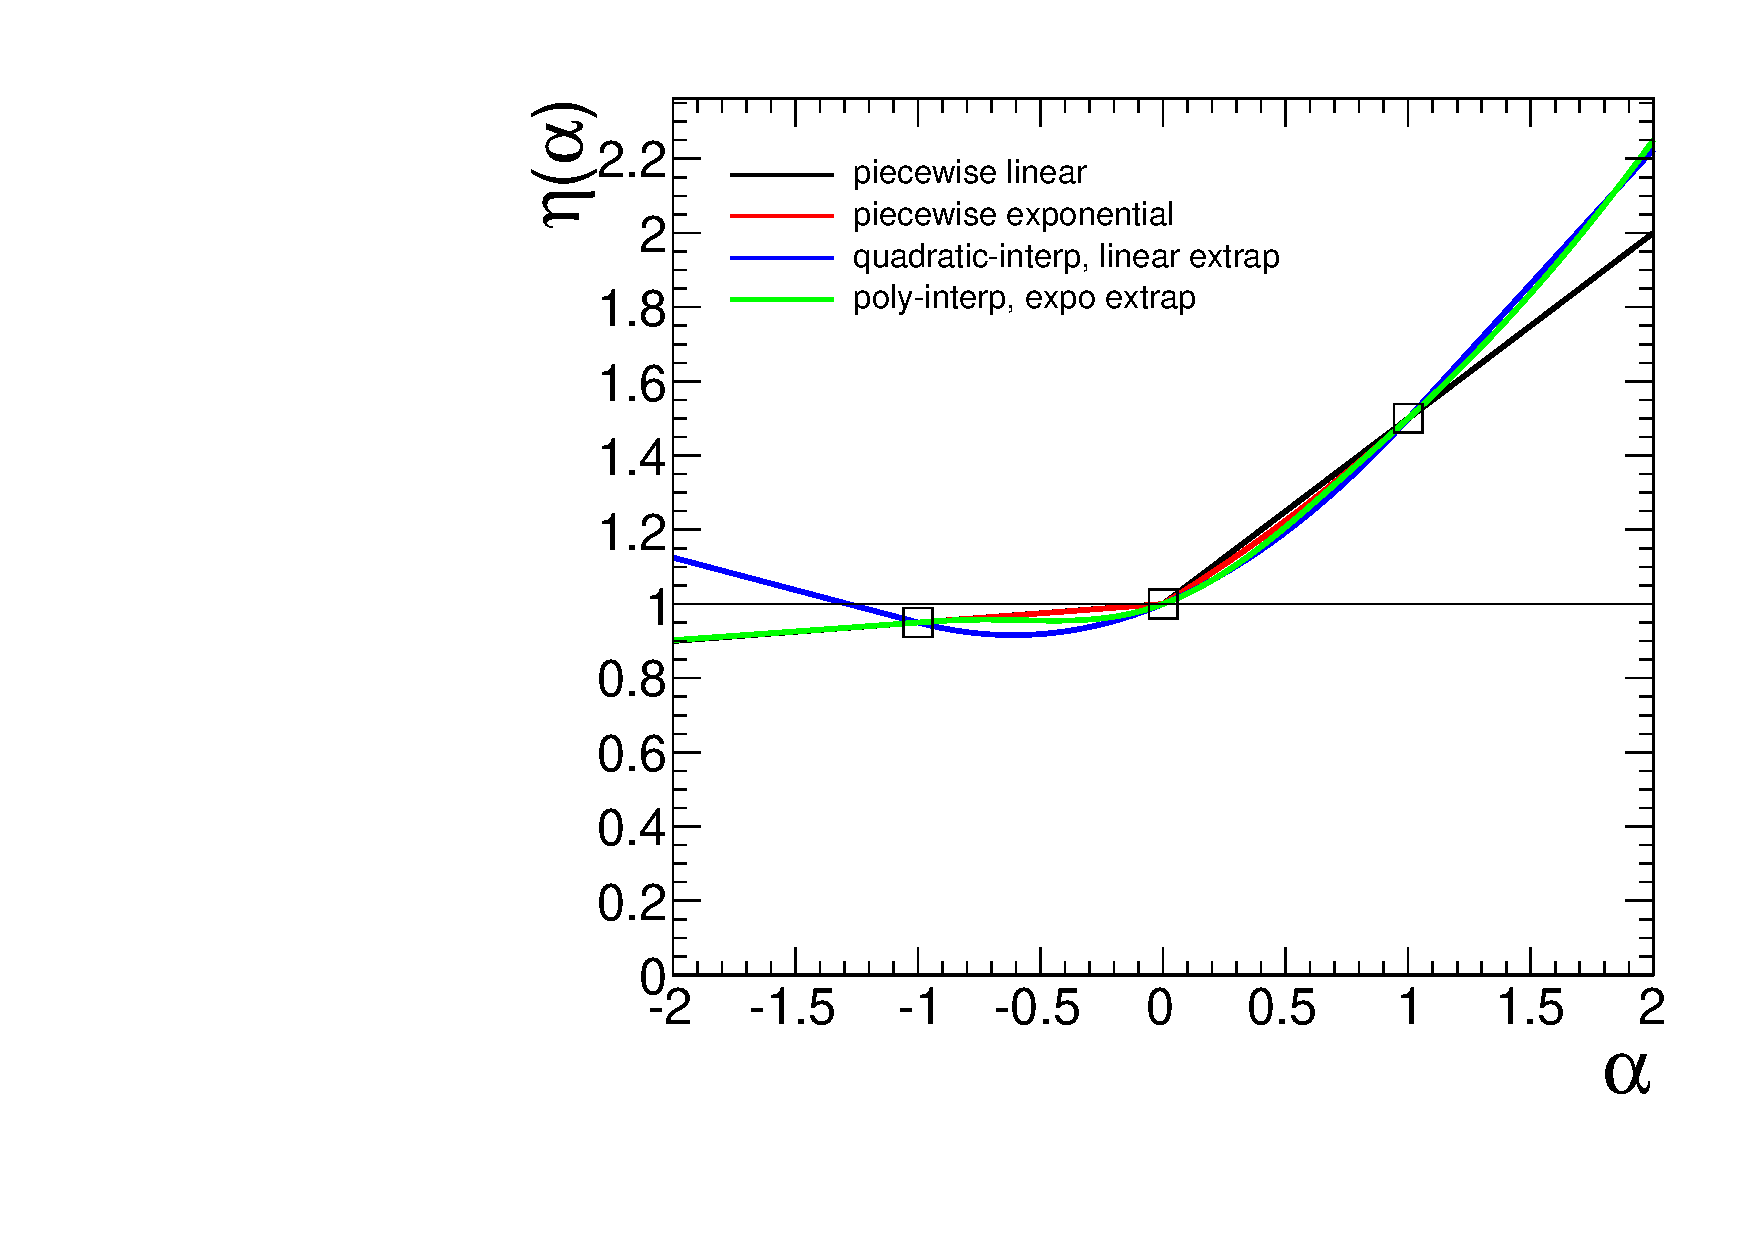
\includegraphics[width=.4\textwidth]{figures/histfactory/interpOption_10_15.pdf}}
\caption{Comparison of the three interpolation options for different $\eta^\pm$.  (a) $\eta^-=0.8$, $\eta^+=1.2$, (b) $\eta^-=1.1$, $\eta^+=1.5$, (c) $\eta^-=0.2$, $\eta^+=1.8$, and (d) $\eta^-=0.95$, $\eta^+=1.5$}
\label{fig:interp1d}
\end{center}
\end{figure}

\begin{figure}[h]
\begin{center}
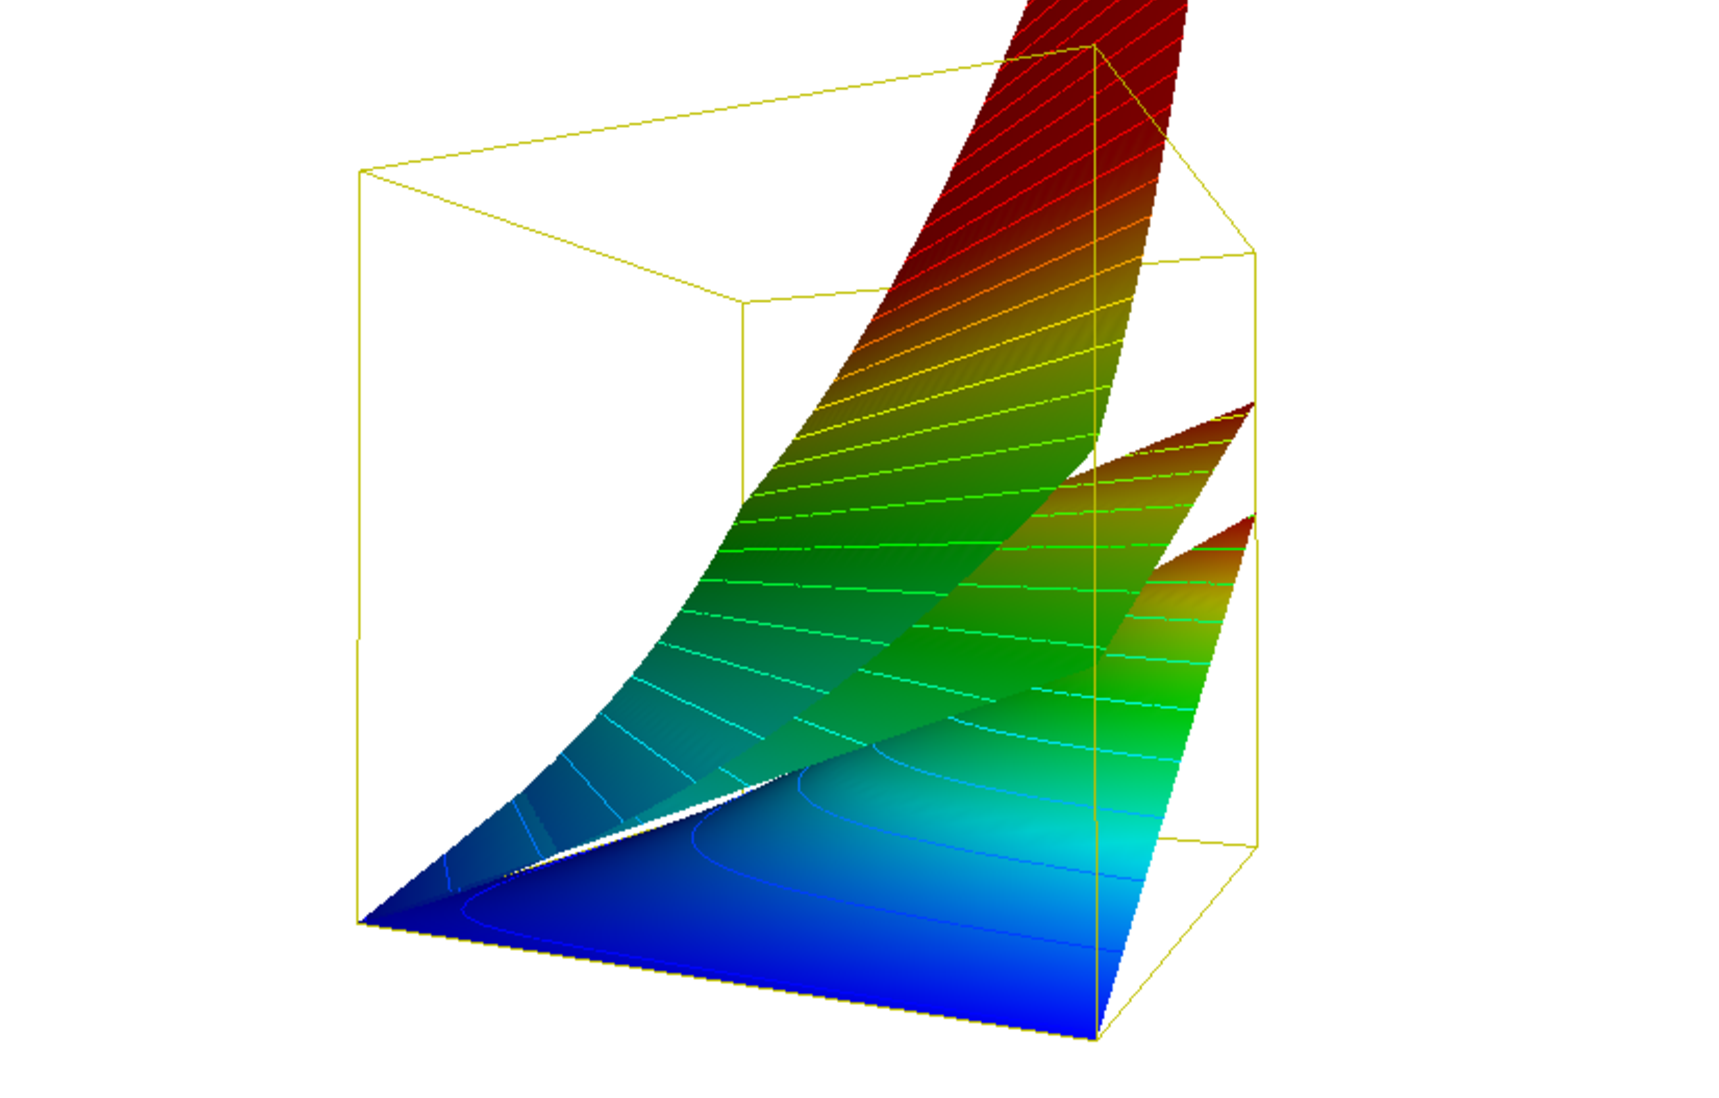
\includegraphics[width=.3\textwidth]{figures/histfactory/Interpolation2d}\hspace{.2\textwidth}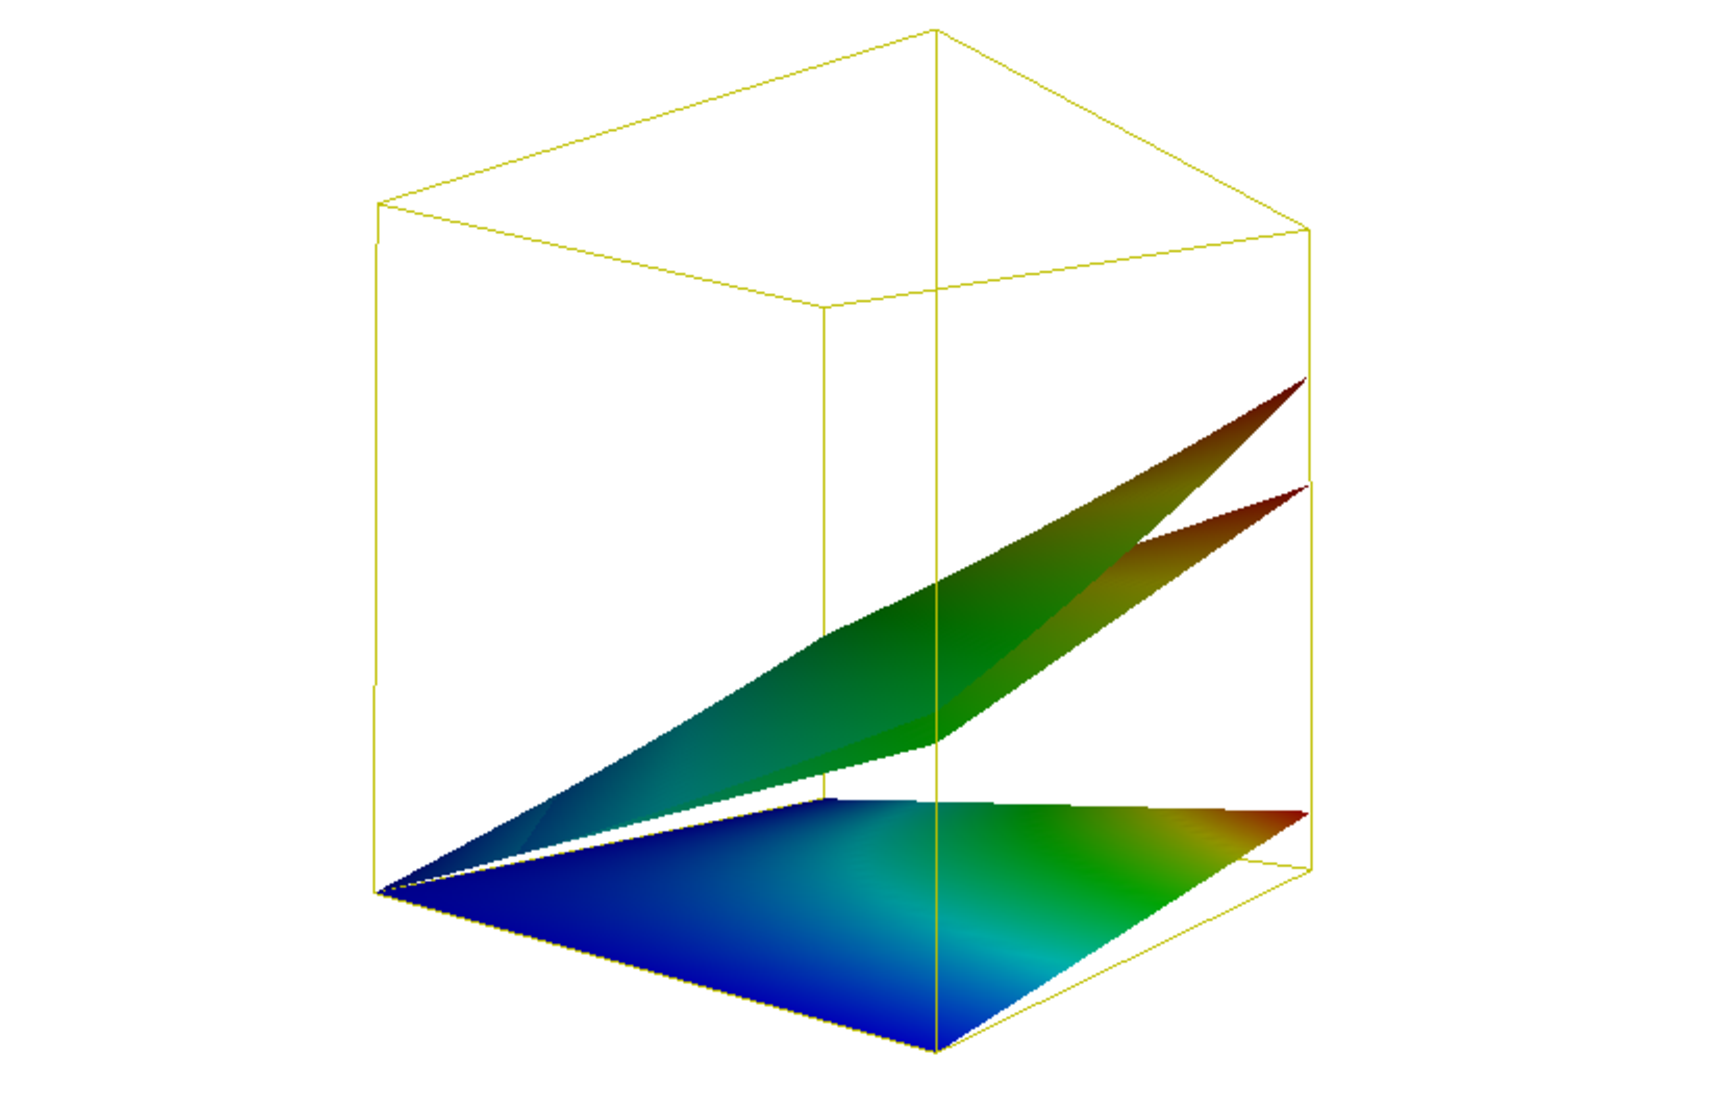
\includegraphics[width=.3\textwidth]{figures/histfactory/Interpolation2d_10}
\caption{The upper-most curve corresponds to $\eta = (\eta^+_1)^{\alpha_1} (\eta^+_2)^{\alpha_2}$ (as in the exponential interpolation option).   The middle surface corresponds to $\eta = 1+\eta^+_1\alpha_1 + \eta^+_2\alpha_2$ (as in the linear interpolation option).  The lowest surface corresponds to $\eta = 1+ \eta^+_1 \alpha_1 \cdot \eta^+_2 \alpha_2$ (currently not an opiton).  The left frame has limits correspond to $\alpha_{1,2} \in [0,3]$ and $\eta(\alpha_1,\alpha_2)\in[0,5]$ and $\eta^+_1=\eta^+_2=1.1$ (eg. a 10\% relative uncertainty). The right frame has limits correspond to $\alpha_{1,2} \in [0,3]$ and $\eta(\alpha_1,\alpha_2)\in[0,5]$ and $\eta^+_1=\eta^+_2=1.5$ (eg. a 50\% relative uncertainty).  }
\label{fig:interp2d}
\end{center}
\end{figure}

\subsubsection{Defaults in ROOT 5.32}

The default strategy for normalization uncertainties $\eta_{s}(\vec{\alpha})$ (ie. \OS\ ) is the piecewise exponential option and it is the standard convention for normalization uncertainties in the LHC Higgs Combination Group.

The default convention for $\sigma_{sb}(\vec{\alpha})$ (ie. \HS\ ) is the piecewise linear option.

The code for $\eta_s(\vec\alpha)$ can be found here:\\
{\tiny \url{http://root.cern.ch/root/html532/src/RooStats__HistFactory__FlexibleInterpVar.cxx.html}}\\
The code for $\sigma_{sb}(\vec\alpha)$ can be found here:\\
{\tiny \url{http://root.cern.ch/root/html532/src/PiecewiseInterpolation.cxx.html}}


\newpage
\subsubsection{Constraint Terms (+ global observables and nuisance parameter priors)}\label{S:constraints}

\subsubsection{Consistent Bayesian and Frequentist modeling}

The variational estimates $\eta^\pm$ and $\sigma^\pm$ correspond to so called ``$\pm 1\sigma$ variations'' in the source of the uncertainty.  Here we are focusing on the source of the uncertainty, not its affect on rates and shapes.  For instance, we might say that the jet energy scale has a 10\% uncertainty.~\footnote{Without loss of generality, we choose to parametrize $\alpha_p$ such that $\alpha_p=0$ is the nominal value of this parameter, $\alpha_p=\pm 1$ are the ``$\pm 1\sigma$ variations''.}  This is common jargon, but what does it mean?  The most common interpretation of this statement is that the uncertain parameter $\alpha_p$ (eg. the jet energy scale) has a Gaussian distribution.  However, this way of thinking is manifestly bayesian.  If the parameter was estimated from an auxiliary measurement, then it is the PDF for that measurement that we wish to include into our probability model.  In the frequentist way of thinking, the jet energy scale has an unknown true value and upon repeating the experiment many times the auxiliary measurements estimating the jet energy scale would fluctuate randomly about this true value.  To aid in this subtle distinction, we use greek letters for the parameters (eg. $\alpha_p$) and roman letters for the auxiliary measurements $a_p$.  Furthermore, we interpret the ``$\pm 1\sigma$'' variation in the frequentist sense, which leads to the constraint term $G(a_p | \alpha_p,1)$.  Then, we can pair the resulting likelihood with some prior on $\alpha_p$ to form a bayesian posterior if we wish.


It is worth mentioning here that the constraint terms are idealized versions of the auxiliary measurements.  In reality, the measurements that were used to estimate the uncertainty in a quantity such as the jet energy scale are actually quite complex.  Ideally, one would include the full likelihood function for those auxiliary measurements into the probability model, but that is often impractical. To the extent that the likelihood resulting from the auxiliary measurement is in the Gaussian regime, then this idealization is not a bad approximation.  

It is often advocated that a ``log-normal'' or ``gamma'' distribution for $\alpha_p$ is more appropriate.    Here we must take some care to build a probability model that can maintain a consistent interpretation in bayesian a frequentist settings.  This will be discussed in the subsections below.  Table~\ref{tab:constraints} summarizes a few consistent treatments of the frequentist pdf, the likelihood function, a prior, and the resulting posterior.

Finally, it is worth mentioning that the uncertainty on some parameters is not the result of an auxiliary measurement -- so the constraint term idealization, it is not just a convenience, but a real  conceptual leap.  This is particularly true for theoretical uncertainties from higher-order corrections or renormalizaiton and factorization scale dependence.  In these cases a formal frequentist analysis would not include a constraint term for these parameters, and the result would simply depend on their assumed values.  As this is not the norm, we can think of reading Table~\ref{tab:constraints} from right-to-left with a subjective Bayesian prior $\pi(\alpha)$ being interpreted as coming from a fictional auxiliary measurement.


\begin{table}[*htb]
\center
\begin{tabular}{llll}
PDF & Likelihood $\propto$ & Prior $\pi_0$ & Posterior $\pi$ \\ \hline
$G(a_p | \alpha_p, \sigma_p)$ & $G(\alpha_p | a_p, \sigma_p)$ & $\pi_0(\alpha_p)\propto$  const & $G(\alpha_p | a_p, \sigma_p)$ \\
$\Pois(n_p | \tau_p \beta_p)$ & $\PGamma(\beta_p | A=\tau_p; B=1+n_p)$ & $\pi_0(\beta_p) \propto$  const & $\PGamma(\beta_p | A=\tau_p; B=1+n_p)$ \\
$\LN(n_p | \beta_p, \sigma_p)$ & $ \beta_p  \cdot \LN(\beta_p | n_p, \sigma_p)$ & $\pi_0(\beta_p) \propto $ const & $\LN(\beta_p | n_p, \sigma_p)$ \\
$\LN(n_p | \beta_p, \sigma_p)$ & $\beta_p  \cdot\LN(\beta_p | n_p, \sigma_p)$ & $\pi_0(\beta_p) \propto 1/\beta_p $  & $\LN(\beta_p | n_p, \sigma_p)$\\
%$G(\ln(a_p) | \ln(\alpha_p), \ln(\sigma_p))$ & $\LN(G(\ln(\alpha_p) | a_p, \sigma_p) = $ & $\pi_0(\alpha_p)\propto$  const & $G(\alpha_p | a_p, \sigma_p)$ \\
\end{tabular}
\caption{Table relating consistent treatments of PDF, likelihood, prior, and posterior for nuisance parameter constraint terms.}
\label{tab:constraints}
\end{table}

%It is common that the uncertainty on a nuisance parameter can be estimated from an auxiliary measurement or from experience, but an explicit probability model relating $\ybf_i$ and $\nu_i$ is not available for practical reasons.  In these cases, it is common to idealize the situation and choose an ad hoc constraint term that summarizes the auxiliary measurement or captures intuition about the uncertainty in the nuisance parameter.  For example, Gaussian constraint terms are very common idealizations of auxiliary measurements.  Here Bayesian reasoning is deceptively natural as one often refers to the prior $\pi(\nu_i)$ in informal conversation without recognizing a Bayesian probability inversion. Similarly, one often refers to a ``Gamma'' prior on a nuisance parameter, which can be interpreted as the posterior resulting from an idealized auxiliary counting experiment with a uniform prior via Bayes theorem: $\pi(\nu_i) \propto \Pois(M|\tau \nu_i) \cdot {\rm Uniform}(\nu_i)$.  In order use a consistent probability model in both frequentist and Bayesian statistical formalisms, it is important to incorporate the Poisson term into the probability model and separate the original uniform prior $\eta(\nu)$ for Bayesian techniques.  Another popular form for an ad hoc constraint term is the log-normal distribution, particularly for non-negative nuisance parameters with large relative uncertainty ($>$20\%).  In this case, one must be more careful about what is assumed to be log-normally distributed.  If one assumes the observable $y$ in the auxiliary measurement is log-normally distributed (as is implied when invoking multiplicative measurement errors) and uses a uniform prior on $\nu_i$ (as in the more familiar Gaussian and Gamma case), then the posterior $\pi(\nu_i)$ does not have a log-normal form.  On the other hand, if one means that the posterior is log-normally distributed, then the likelihood function and prior must be specified to provide a consistent frequentist treatment of the problem.  While a $\eta(\nu_i) \propto 1/\nu_i$ prior allows both the PDF and the posterior to have a log-normal form, the likelihood function and the posterior are no longer proportional (as they were in the Gaussian and Gamma case).  The lesson here is that one cannot simply appeal to idealized measurements when and hope for an unambiguous interpretation when there are large uncertainties involved.

\subsubsection{Options for Constraint Terms}


\flushleft{\bf Gaussian Constraint}

The Gaussian constraint for $\alpha_p$ corresponds to the familiar situation.  It is a good approximation of the auxiliary measurement when the likelihood function for $\alpha_p$ from that auxiliary measurement has a Gaussian shape.  More formally, it is valid when the maximum likelihood estimate of $\alpha_p$ (eg. the best fit value of $\alpha_p$) has a Gaussian distribution.  Here we can identify the maximum likelihood estimate of $\alpha_p$ with the global observable $a_p$, remembering that it is a number that is extracted from the data and thus its distribution has a frequentist interpretation.  In the RooFit workspace produced by \HF, this variable has a name like \texttt{nom\_alpha\_<name>} and it is included in the \texttt{ModelConfig}'s list of \texttt{GlobalObservables}.  We chose to scale $\alpha_p$ (and thus $a_p$ so that the distribution has unit variance: $G(a_p | \alpha_p,1)$.  Note that if we assume the true value $\alpha_p\ne0$ and we sample $a_p$ via (toy) Monte Carlo techniques, the distribution of $a_p$ will not have a mean of 0.
\begin{equation}
G(a_p | \alpha_p, \sigma_p) = \frac{1}{\sqrt{2\pi \sigma_p^2}} \exp \left[ -\frac{(a_p - \alpha_p)^2}{2\sigma_p^2} \right]
\end{equation}
with $\sigma_p=1$ by default.

Note that the PDF of $a_p$ and the likelihood for $\alpha_p$ are positive for all values.  Thus if $\alpha_p$ represents a shifted and rescaled version of a more physical parameter that is bounded, then the Gaussian distribution is attributing some positive probability to the unphysical regions.  For instance, energy scales, reconstruction efficiencies, and background normalizations must be $\ge 0$. Consider a jet energy scale that is estimated with 25\% uncertainty, then $\alpha<-4$ would correspond to an unphysical negative jet energy scale.  One can also consider normalization uncertainties where $\alpha$ and $\eta(\alpha)$ are more directly related -- in particular $\eta(\alpha)$ is a linear function.  Consider a background that is estimated with 50\% uncertainty, then for $\alpha<-2$ will correspond to a negative background estimate, and we will have $\eta(\alpha<2)<0$.

Technically, RooFit's PDF classes (\texttt{RooGaussian} in this case) make sure that the PDF is normalized to unity within the range of the observable (in this case $a_p$).  So the technical implementation will actually correspond to a truncated and renormalized Gaussian (the default range for $a_p$ is $[-5,5]$).  


\flushleft{\bf Poisson (``Gamma'') constraint}

When the auxiliary measurement is actually based on counting events in a control region (eg. a Poisson process), a more accurate to describe the auxiliary measurement with a Poisson distribution.  It has been shown that the truncated Gaussian constraint can lead to undercoverage (overly optimistic) results, which makes this issue practically relevant.  Table~\ref{tab:constraints} shows that a Poisson PDF together with a uniform prior leads to a gamma posterior, thus this type of constraint is often called a ``gamma'' constraint.  This is a bit unfortunate since the gamma distribution is manifestly Bayesian and with a different choice of prior, one might not arrive at a gamma posterior.  When dealing with the Poisson constraint, it is no longer convenient to work with  our conventional scaling for $\alpha_p$ which can be negative.  Instead, it is more natural to think of the number of events measured in the auxiliary measurement $n_p$ and the mean of the Poisson parameter.  This information is not usually available, instead one usually has some notion of the relative uncertainty in the parameter $\sigma_p^{\rm rel}$ (eg. a the jet energy scale is known to 10\%).  In order to give some uniformity to the different uncertainties of this type and think of relative uncertainty, the nominal rate is factored out into a constant $\tau_p$ and the mean of the Poisson is given by $\tau_p \beta_p$.  
\begin{equation}
\Pois(n_p | \tau_p \beta_p) =\frac{ (\tau_p \beta_p)^{n_p} \; e^{-\tau_p \beta_p} } {n_p!}
\end{equation}
Here we can use the fact that Var$[n_p]=\sqrt{\tau_p\beta_p}$ and reverse engineer the nominal auxiliary measurement 
\begin{equation}
n_p^0 =  \tau_p = (1/\sigma_{p}^{\rm rel})^2\; .
\end{equation}
where the superscript $0$ is to remind us that $n_p$ will fluctuate in repeated experiments but $n_p^0$ is the value of our measured estimate of the parameter.

Thus the nominal situation corresponds to $\beta_p=1$ and the ``$\pm 1\sigma$ variations'' (which is now ambiguous) conventionally correspond to $\beta_p=1\pm \sigma_p^{\rm rel} = 1\pm \tau_p^{-\onehalf}$.   It is more convenient to modify the constraint term while keeping the interpolation $\eta(\alpha)$ fixed, thus we introduce the linear relationship that satisfies $\alpha(\beta=1)=0$ and $\alpha(\beta=1\pm \tau_p^{-\onehalf})=\pm 1$
\begin{equation}
\alpha_p(\beta_p) = \sqrt{\tau_p}\,(\beta_p -1)
%\alpha_p(\beta_p) = \sqrt{1+1/\sigma_p^2}(\beta_p -1) %in 5.32 this is the code
\end{equation}

One important thing to keep in mind is that there is only one constraint term per nuisance parameter, so there must be only one $\sigma_p^{rel}$ per nuisance parameter.  This $\sigma_p^{rel}$ is related to the fundamental uncertainty in the source and we cannot infer this from the various response terms $\eta_{ps}^\pm$ or $\sigma_{pub}^\pm$.  In the XML this is not a property of a channel, but of a measurement and it is encoded in a term like 
{\tiny
%\begin{lstlisting}[language=XML]
   <ConstraintTerm Type="Gamma" RelativeUncertainty="0.1">JES</ConstraintTerm>
%\end{lstlisting}
}

Another technical difficulty is that the Poisson distribution is discrete. So if one were to say the relative uncertainty was 30\%, then we would find $n_p^0=11.11...$, which is not an integer.  Rounding $n_p$ to the nearest integer while maintaining $\tau_p= (1/\sigma_{p}^{\rm rel})^2$ will bias the maximum likelihood estimate of $\beta_p$ away from 1.  As of ROOT 5.32 the \texttt{ConstraintTerm Type="Gamma"} used the \texttt{RooGamma} (which generalizes more continuously) with 
\begin{equation}
\PGamma(\beta_p | A=\tau_p, B=n_p-1) = A (A \beta_p)^{B} e^{-A \beta_p} / \Gamma(B)
\end{equation}
The implementation works fine for likelihood fits, bayesian calculations, and frequentist techniques based on asymptotic approximations, but it does not offer a consistent treatment of the pdf for the global observable $n_p$ that is needed for techniques based on Monte Carlo techniques.  In future versions of ROOT, the constraint will probably be replaced with \texttt{RooPoisson} with an option \texttt{setNoRounding(true)}.


%it->first.c_str(),-1./scale,1./scale))
%      double scale = 1/sqrt((1+1/pow(relativeUncertainty,2)));

\flushleft{\bf Log-normal constraint}

From Eadie et al., ``The log-normal distribution represents a random variable whose logarithm follows a normal distribution. It provides a model for the error of a process involving many small multiplicative errors (from the Central Limit Theorem). It is also appropriate when the value of an observed variable is a random proportion of the previous observation.''

As in the case of the ``Gamma'' constraints we need to reparametrize to a nuisance parameter $\beta_p$ that is positive and centered around 1.  Again we use $\alpha$ for the response of the systematics and relate the two via
\begin{equation}
\alpha_p(\beta_p) = \sqrt{\tau_p}\,(\beta_p -1)
\end{equation}
And the equivalent global observable is
\begin{equation}
n_p^0 =  \tau_p = (1/\sigma_{p}^{\rm rel})^2\; .
\end{equation}
{\tiny
%\begin{lstlisting}[language=XML]
   <ConstraintTerm Type="LogNormal" RelativeUncertainty="0.1">JES</ConstraintTerm>
%\end{lstlisting}
}


\begin{equation}
\LN(n_p | \beta_p, \kappa_p) = \frac{1}{\sqrt{2\pi}\ln \kappa}\frac{1}{n_p} \exp \left[ -\frac{\ln(n_p/ \beta_p)^2}{2(\ln \kappa_p)^2} \right]
\end{equation}
(blue curve in Fig.~\ref{fig:lognormal}(a)).
\begin{equation}
L( \beta_p) = \frac{1}{\sqrt{2\pi}\ln \kappa}\frac{1}{n_p} \exp \left[ -\frac{\ln(n_p/ \beta_p)^2}{2(\ln \kappa_p)^2} \right]
\end{equation}
(red curve in Fig.~\ref{fig:lognormal}(b)).
\begin{equation}
\pi( \beta_p) \propto \pi_0(\beta_p)  \; \frac{1}{\sqrt{2\pi}\ln \kappa}\frac{1}{n_p} \exp \left[ -\frac{\ln(n_p/ \beta_p)^2}{2(\ln \kappa_p)^2} \right]
\end{equation}
When paired with an ``ur-prior'' $\pi_0(\beta_p) \propto 1/\beta_p$ (green curve in Fig.~\ref{fig:lognormal}(b)), this results in a posterior distribution that is also of a log-normal form for $\beta_p$ (blue curve in Fig.~\ref{fig:lognormal}(b)).



\begin{figure}[htbp]
\begin{center}
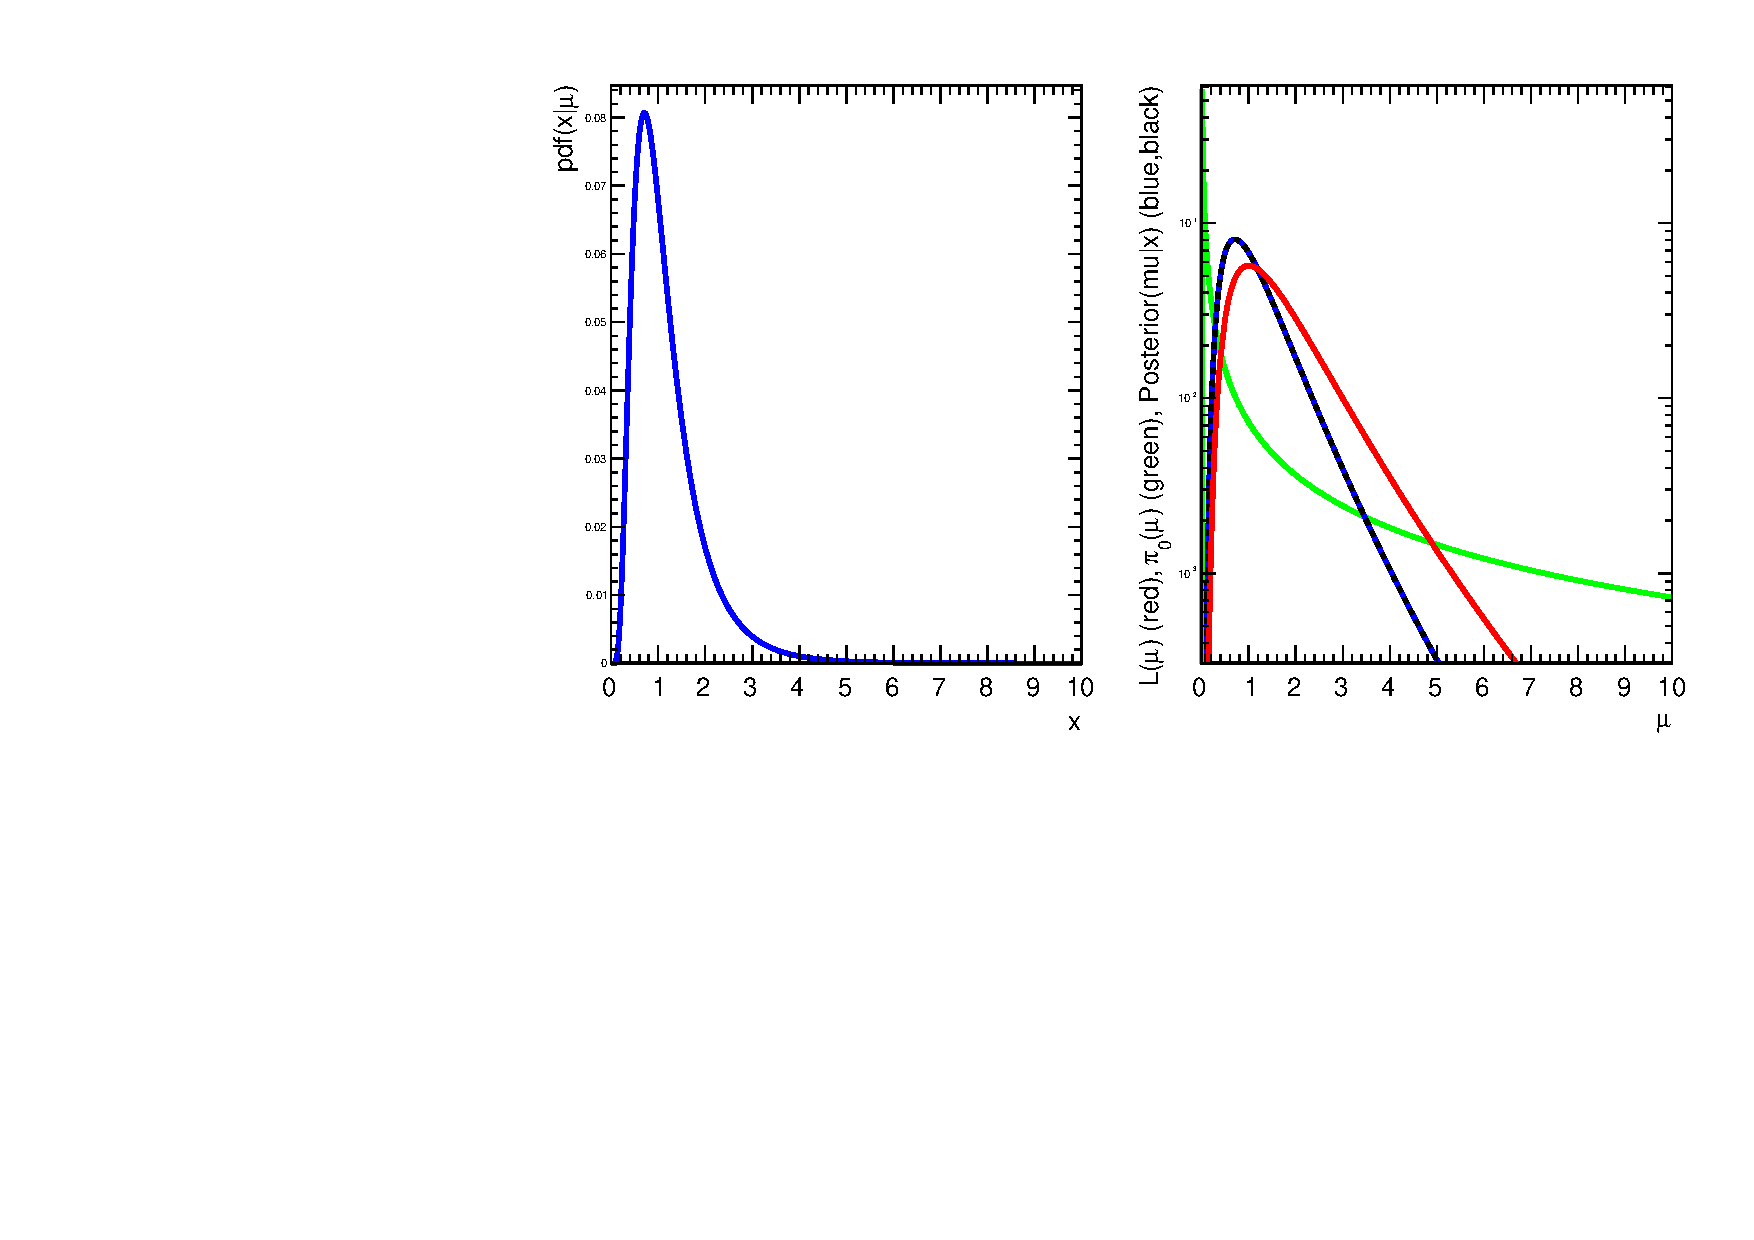
\includegraphics[width=.4\textwidth]{figures/histfactory/lognormal}
\caption{The lognormal constraint term: (left) the pdf for the global observable $a_p$ and (right) the likelihood function, the posterior based on a flat prior on $\beta_p$, and the posterior based on a $1/\beta_p$ prior.}
\label{fig:lognormal}
\end{center}
\end{figure}


\newpage

\subsection{Examples}
\subsubsection{A Simple Example}

Here we consider a single channel example with one signal and two backgrounds.  All three samples histograms are based on theoretical predictions (aka. Monte Carlo), thus the luminosity uncertainty should propagate to these channels --  this is accomplished by \texttt{NormalizeByTheory="True"}.  In this example, no shape uncertainties are included and statistical uncertainty on the histograms is not taken into account.  The parameter of interest in this example is the signal cross section relative to the predicted value used to create the signal histogram -- it is called \texttt{SigXsecOverSM}.  Three systematic effects are considered that modify the normalization on the channels -- here just named ``syst1'', ``syst2'', and ``syst3''.  In this example syst3 affects the normalization of both backgrounds (though in opposite directions).

\begin{table}[h]
\center
\begin{tabular}{l | c c c}
Syst & Signal ($s$=1) & Background1 ($s$=2)& Background2 ($s$=2)\\ \hline
syst1 ($p=1$) & $\eta_{11}^+=1.05$, \;$\eta_{11}^-=0.95$ & -- & -- \\
syst2 ($p=2$)& -- & $\eta_{22}^+=1.07$, \;$\eta_{22}^-=0.93$ & -- \\
syst3 ($p=3$)& -- &  $\eta_{32}^+=1.03$, \;$\eta_{32}^-=0.95$   & $\eta_{33}^+=0.97$, \;$\eta_{33}^-=1.02$ \\
\end{tabular}
\caption{Tabular representation of sources of uncertainties that produce a correlated effect in the normalization individual samples (eg. OverallSys).  The $\eta^+_{ps}$ represent histogram when $\alpha_s=1$ and are inserted into the \texttt{High} attribute of the \OS\  XML element.  Similarly, the $\eta^-_{ps}$ represent histogram when $\alpha_s=-1$ and are inserted into the \texttt{Low} attribute of the \OS\  XML element. Note, this does not imply that $\eta^+ > \eta^-$, the $\pm$ superscript correspond to the variation in the source of the systematic, not the resulting effect.}
\end{table}


\newpage

%
%{\tiny
%\lstinputlisting[]{../../roostats/sandbox/histfactorySandbox/testStdDemos/config/HistFactorySchema.dtd}
%}



One can convert this Gaussian constraints into a Poisson/Gamma systematic by adding lines like
{\tiny
%\begin{lstlisting}[language=XML]
   <ConstraintTerm Type="Gamma" RelativeUncertainty="0.1">JES</ConstraintTerm>
%\end{lstlisting}
}
to the {\tt Measurement} element.  


\subsection{C++ and Python}
